% Chapter X

\chapter{Anomaly Detection in Distributed Tracing Data} % Chapter title
\label{ch:traces} % For referencing the chapter elsewhere, use \autoref{ch:name} 
\minitoc
\bigskip

Distributed traces contain information about the execution workflow and performance at a service level within the system. The trace representation, noise, large number of services, complex service relationships between them, arbitrary lengths, and lack of labels pose difficulties for the anomaly detection methods~\cite{liu2020unsupervised}. In this chapter, to address these challenges, we introduce a sequential representation of the trace. This helps utilize various methods for anomaly detection in sequential data. We describe a baseline approach based on sequence prediction with LSTMs to perform anomaly detection~\footnote{Based on our early study on trace anomaly detection using deep learning~\cite{nedelkoski2019anomalymultimodal}}. This modeling approach has several advantages and limitations, identified in this chapter. We reformulate the learning task from sequence prediction to prediction of missing parts of the trace. This helps preserve the major advantages of sequential trace representation and increase the robustness to previous limitations such as the noise and degraded performance on larger traces. Finally, we demonstrate the ability of the method for root-cause localization, i.e., finding the contribution of each of the services within the trace to the decision whether the trace is anomalous.

This chapter includes the following contributions~\footnote{Parts of this chapter are published in ~\cite{nedelkoski2019anomalymultimodal,nedelkoski2020data,nedelkoski2019anomaly,nedelkoski2020selftracing} and a patent is filed in~\cite{nedelkoski2020patentjasmin}.}.
\begin{itemize}
    \item We compile the trace structure as a text sequence, which provides possibilities for applications of deep learning methods.
    \item We introduce a baseline deep learning approach based on LSTMs.
    \item We present a problem formulation for anomaly detection in distributed tracing and method based on self-supervised learning, denoted as Tracy.
    \item We demonstrate an approach to utilize the model to track the differences between the normal and abnormal traces. This leads to an improved reasoning for the root cause analysis and localization of the services with downgraded performances.
\end{itemize}

\section{Sequence learning for trace anomaly detection}
In this section, we start with transformation of the trace to a textual representation and describe the preprocessing steps needed for the model learning phase. We present a baseline LSTM-based approach and derive key benefits and drawbacks. These insights are utilized to reformulate the autoregressive problem definition and design Tracy, a self-supervised trace anomaly detection method. 

\subsection{Trace preprocessing}
Traces are produced by a program that executes a set of logic and control functions, following certain patterns and grammar rules on which the system operates. If the spans of the trace are sorted by time, the graph-like trace structure can be expressed as a finite sequence, $T=(S_1, \dots, S_m)$. We transform and compile the trace to such representation and provide an analogy to the natural language. A trace can be related to a sentence, the events/spans inside a trace to words, and the causal relationship between events to a language grammar (e.g., relations between words).

\begin{figure}[!htbp]
\centerline{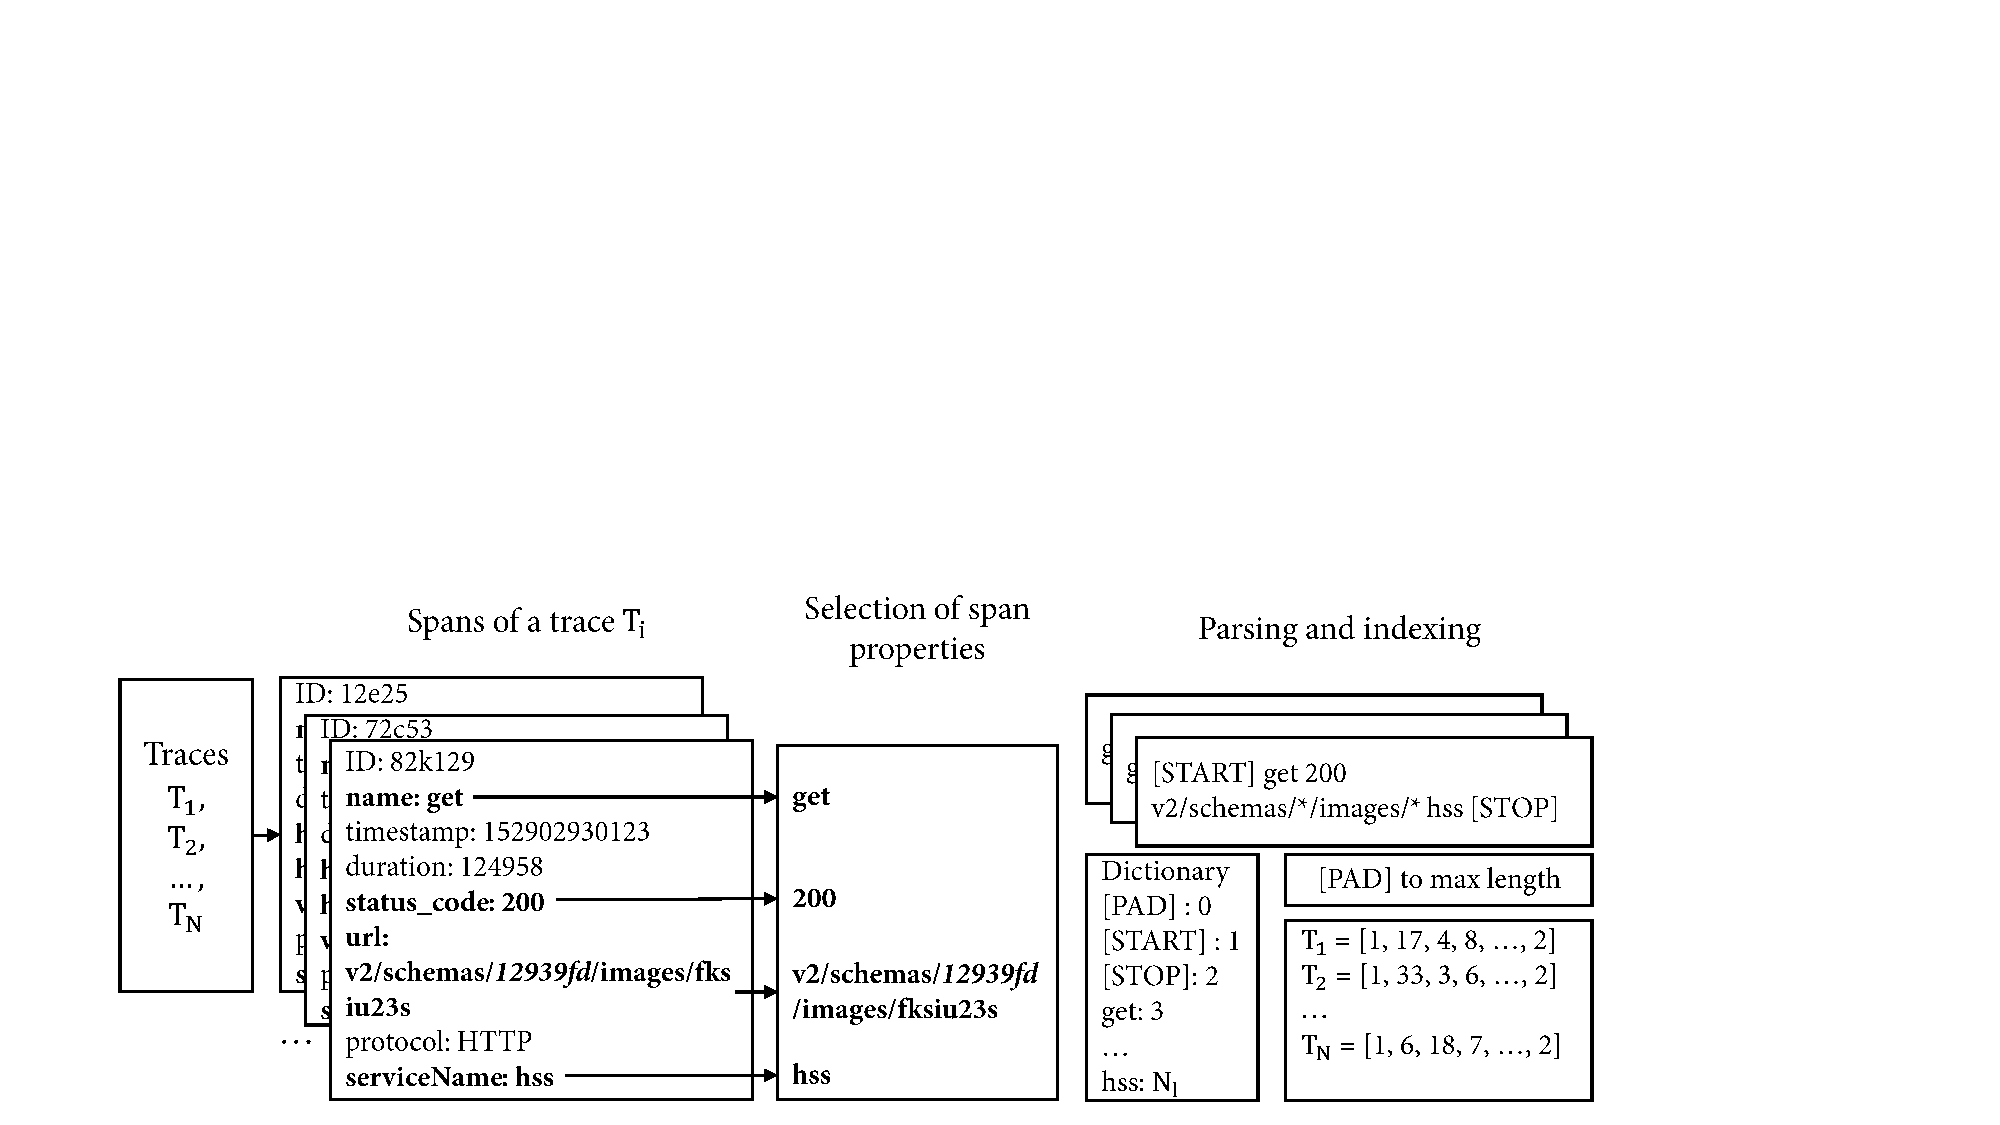
\includegraphics[width=1.0\textwidth]{gfx/chap6/tracepreprocessing.pdf}}
\caption{Preprocessing of the trace.}
\label{fig:tracepreprocessing}
\end{figure}

As the spans contain an additional meta-information, they have to be parsed to obtain a uniform structure, before they can be effectively used for anomaly detection~\cite{nedelkoski2019anomaly}. The parsing, similar to that for logs, uses raw spans as an input and generates a template. Thus, the trace can be represented as a sequence of template indices.

In Figure~\ref{fig:tracepreprocessing}, we show the parsing procedure of the trace's spans. Depending on the span type (e.g., initiated from RPC or HTTP request), we select only the most important part properties. They, in the example of HTTP request, are the name of the method (e.g., GET), HTTP status code, URL, and service name. The importance of the properties is related to their informativeness. Properties that are different in each span, e.g., the ID of the span, are not considered as informative properties.

Considering the large variability of the URLs, owing to mostly the IDs inside them, the number of different spans can be very large, leading to difficulties in modeling. As most of these span's URLs representing one service differ solely in the identifiers (e.g., the ID 12939fd is ID of the image), we replace them with $\langle * \rangle$ through parsing and extract span templates or groups. To this end, we use a log parsing method (NuLog). At this point, the trace is represented as a sequence of span templates. As traces can contain repetitive spans, to preserve the start and end of the trace, we add two additional spans to the beginning and end of the trace ([START] and [STOP]). 

The third step in the prepossessing is the creation of a lookup table where the templates that are output from the parser are mapped to a specific index. Thus, each span is mapped to an index and the trace is a sequence of indices. To consider the possibly different lengths of the traces, the traces are padded up to $max\_len$. This parameter represents the maximum allowed trace length. This makes the traces equally sized. The data format at the output of the preprocessing has a shape of $D_1 = (N_t, max\_len)$, where each row is a trace $T_i = \{x_1^i,x_2^i,\dots, x_{max\_len}\}$, $N_t$ is the number of all recorded traces, and $x_j^i \in \mathbb{V}$ are indices from the dictionary. 

\begin{figure}[!t]
\centerline{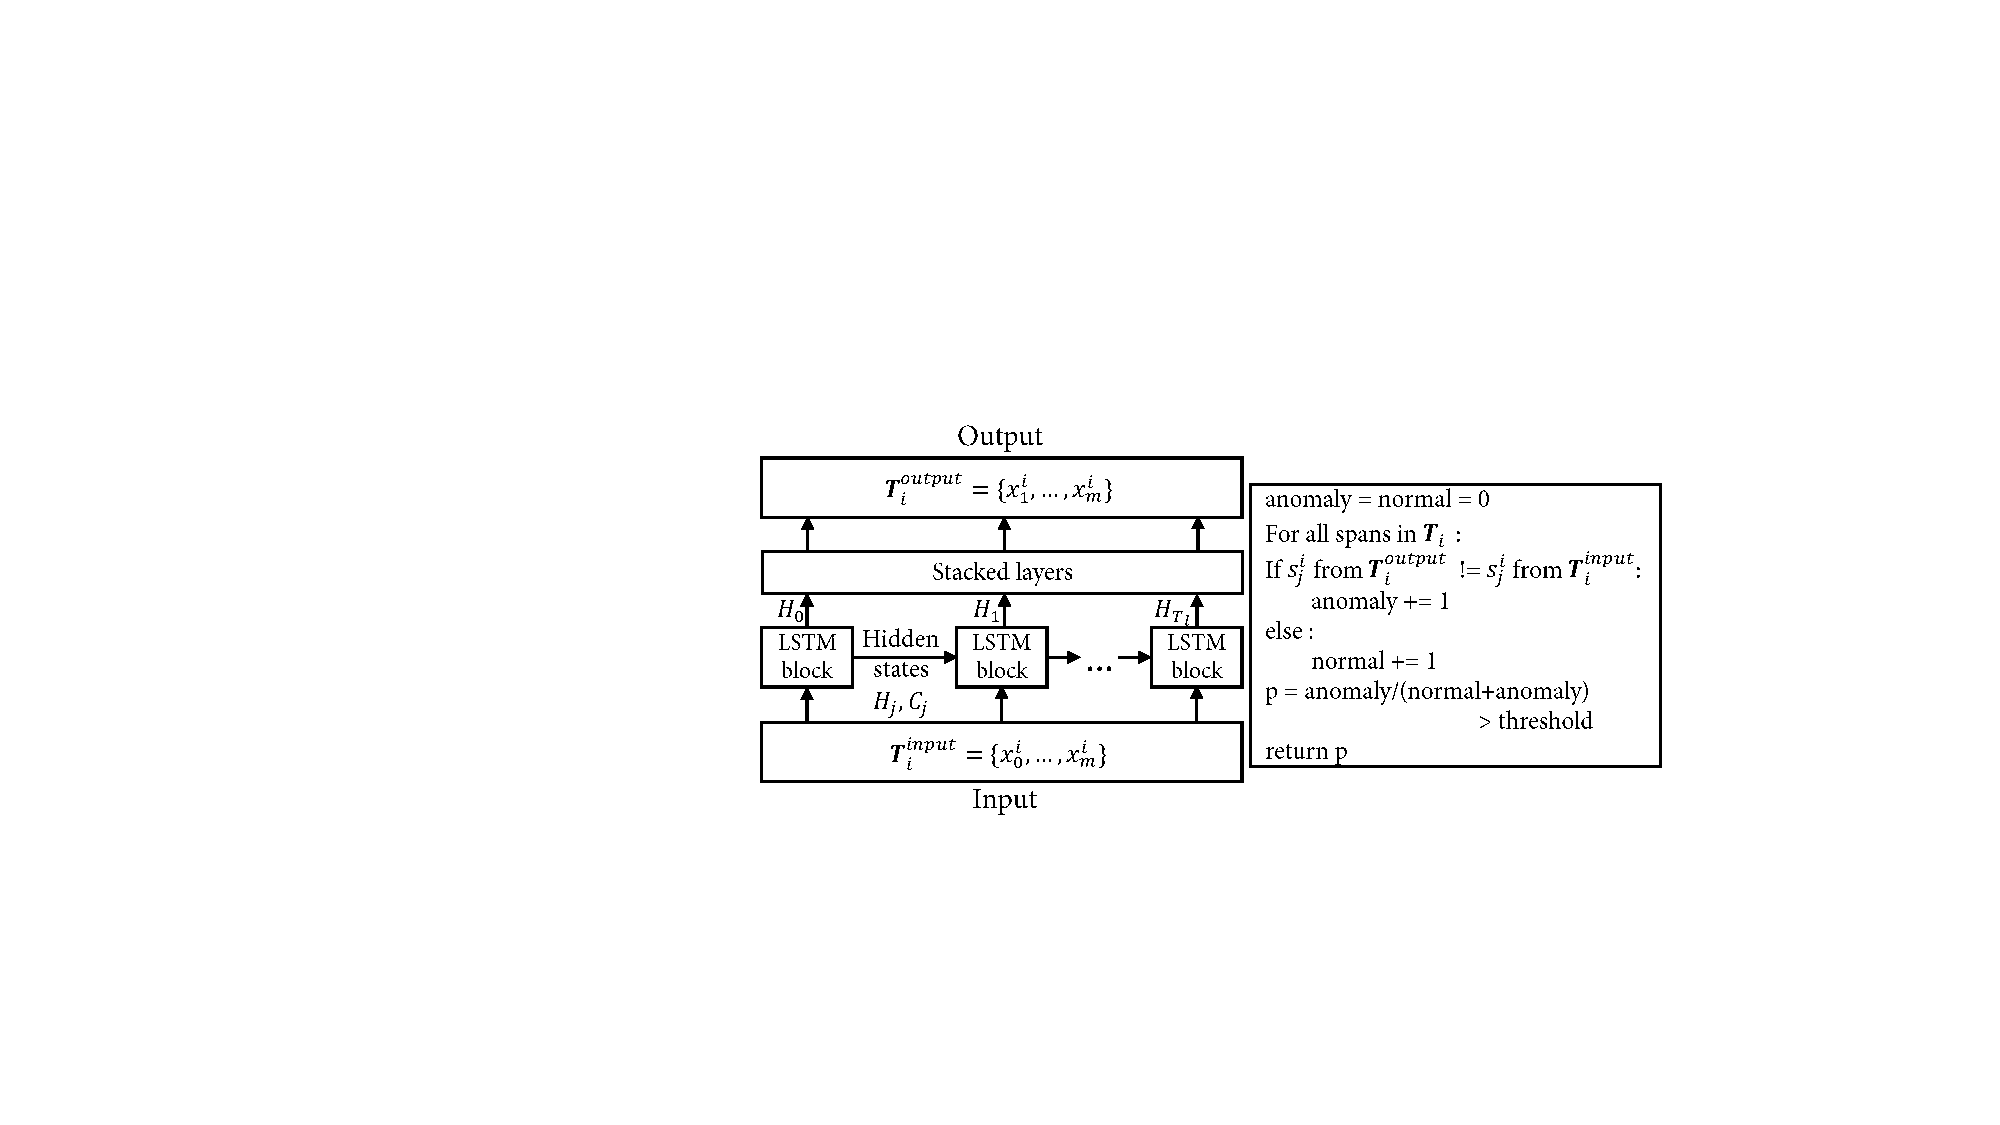
\includegraphics[width=1.0\textwidth]{gfx/chap6/lstmprocesstrace.pdf}}
\caption{LSTM network architecture for trace anomaly detection.~\cite{nedelkoski2019anomalymultimodal}}
\label{fig:lstmtraceprocess}
\end{figure}

\subsection{Autoregressive LSTM-based method for anomaly detection}
To perform anomaly detection, we start by modeling the normal system behavior. We model the transition probability from a sequence of spans into the next in-sequence span
\begin{equation}
     P(x_t=l_i|\{x_{t-h}, \dots, x_{t-2}, x_{t-1}\}),
\end{equation}
where $P$ is the conditional probability of the next span for given input
recent sequence of $h$ spans within the trace and $l_i \in L=\{l_0, l_1, \dots, l_{N_l}\}$ is the index from the dictionary of spans. The conditional probability can be modeled with an RNN, e.g, LSTM/GRU. We show the architecture of the approach in Figure~\ref{fig:lstmtraceprocess}.

The input to the model are the indices from the spans. Each $x_t$ is fed as an input in the corresponding timestep $t$. The output at $t$, for the current inputs $\{x_{t-h}, \dots, x_{t-2}, x_{t-1}\}$, is a probability distribution over the $N_l$ unique labels from $L$. 
Every LSTM block at $t$ is composed of $H$ LSTM cells. 
It has a memory state that encodes all information from the previous timesteps together with the input fed at the same timestep.

The vertical stacking of layers is a common practice to achieve better results by extracting highly-abstract features~\cite{Hundman:2018:DSA:3219819.3219845,vincent2010stacked}. The model's parameters are optimized by minimizing the categorical cross-entropy loss between the predicted span and ground truth.

During the prediction time, if we are unable to successfully predict a certain number of next spans (more than a specified threshold), the trace is considered anomalous; otherwise, it is normal.

\subsection{Limitations of autoregressive approaches}
The LSTM-based method belongs to the autoregressive approaches. Thus, it has several inherit limitations including (1) forward context is not considered during the modeling phase~\cite{devlin2018bert}. Thus, the model does not utilize the full trace information. (2) Lack of robustness to noise and trace length variability, owing to the inability of autoregressive models to preserve long interdependencies between the services (e.g., the span on the first position is related to the span on the 100-th position of the trace). Moreover, as mentioned above, the sequential representation of the trace is obtained using the initially graph-like trace structure. Therefore, this representation does not preserves all initial information. 

A desired behavior of the model would be to learn additional interdependencies between the spans in the trace, other than the sequential. The model, to preserve the graph information within the sequence, needs to extract dependencies between distant spans in the sequence. For example, as depicted in Figure~\ref{fig:interdependenciessequential}, the model needs to be able to infer that span A is related to span K, which have long-term dependencies. To address these limitations of autoregressive models, we reformulate the learning task and present a novel method, Tracy.


\begin{figure}[!t]
\centerline{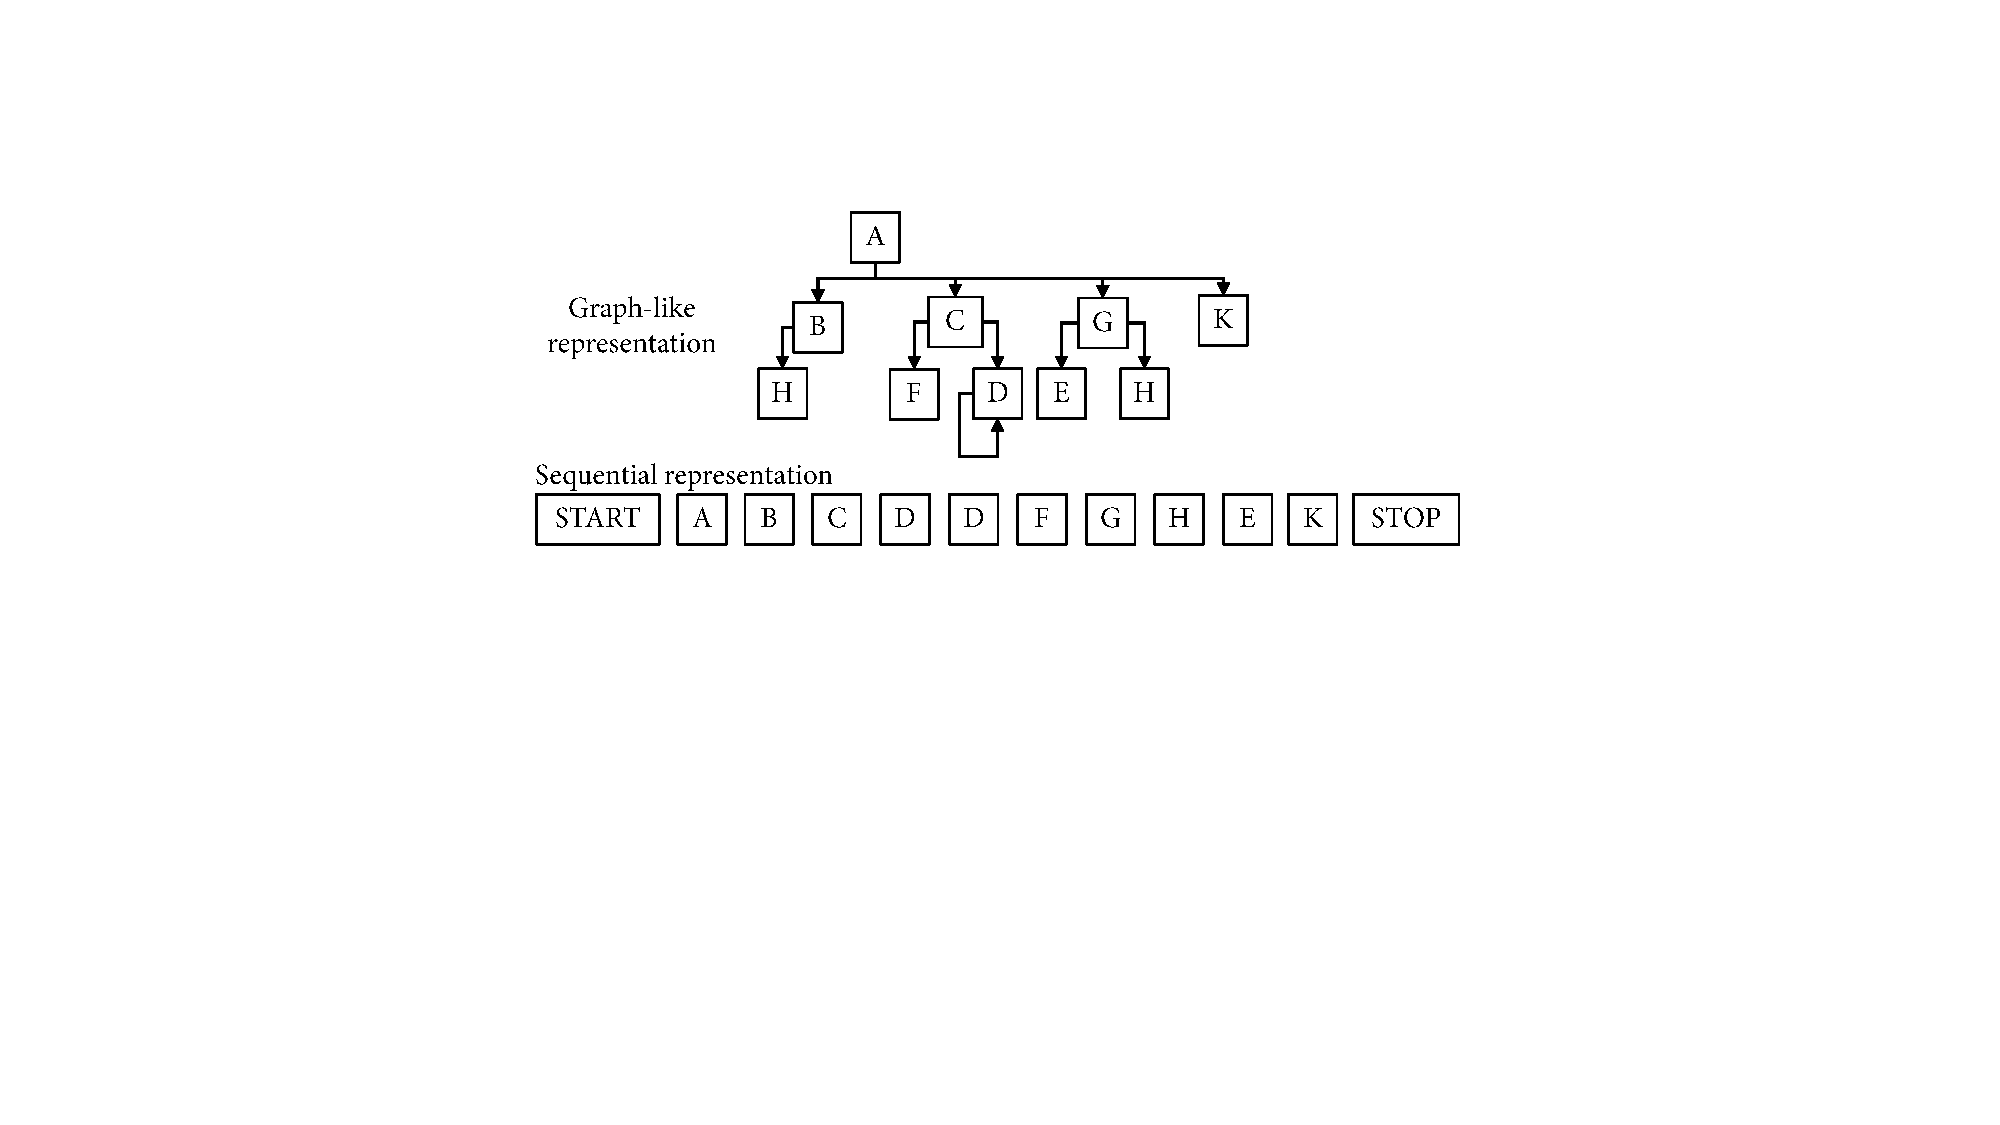
\includegraphics[width=1.0\textwidth]{gfx/chap6/interdependenciessequential.pdf}}
\caption{Long term interdependencies.}
\label{fig:interdependenciessequential}
\end{figure}


\section{\textit{Tracy}: self-supervised anomaly detection in distributed traces}
Each span's position within the trace is dependent on the other spans (can be located at any position) in the trace~\cite{sigelman2010dapper,RepTrace,chow2014mystery}. The contextual information is related to the likelihood of occurrence of a particular span on a position within that trace. The set of spans used to pinpoint the location of another span is referred to as context of the span. Intuitively, it is reasonable that deep models, e.g., Bi-LSTM~\cite{huang2015bidirectional}), are strictly more powerful than either a left-to-right (autoregressive) model or shallow concatenation of left-to right and right-to-left models. However, standard conditional models can only be trained left-to-right or right-to-left, as bidirectional conditioning would allow each word to indirectly "see itself" and the model could trivially predict the target word in a multi-layered context, which would lead to over-fitting.

\begin{figure}[!t]
\centerline{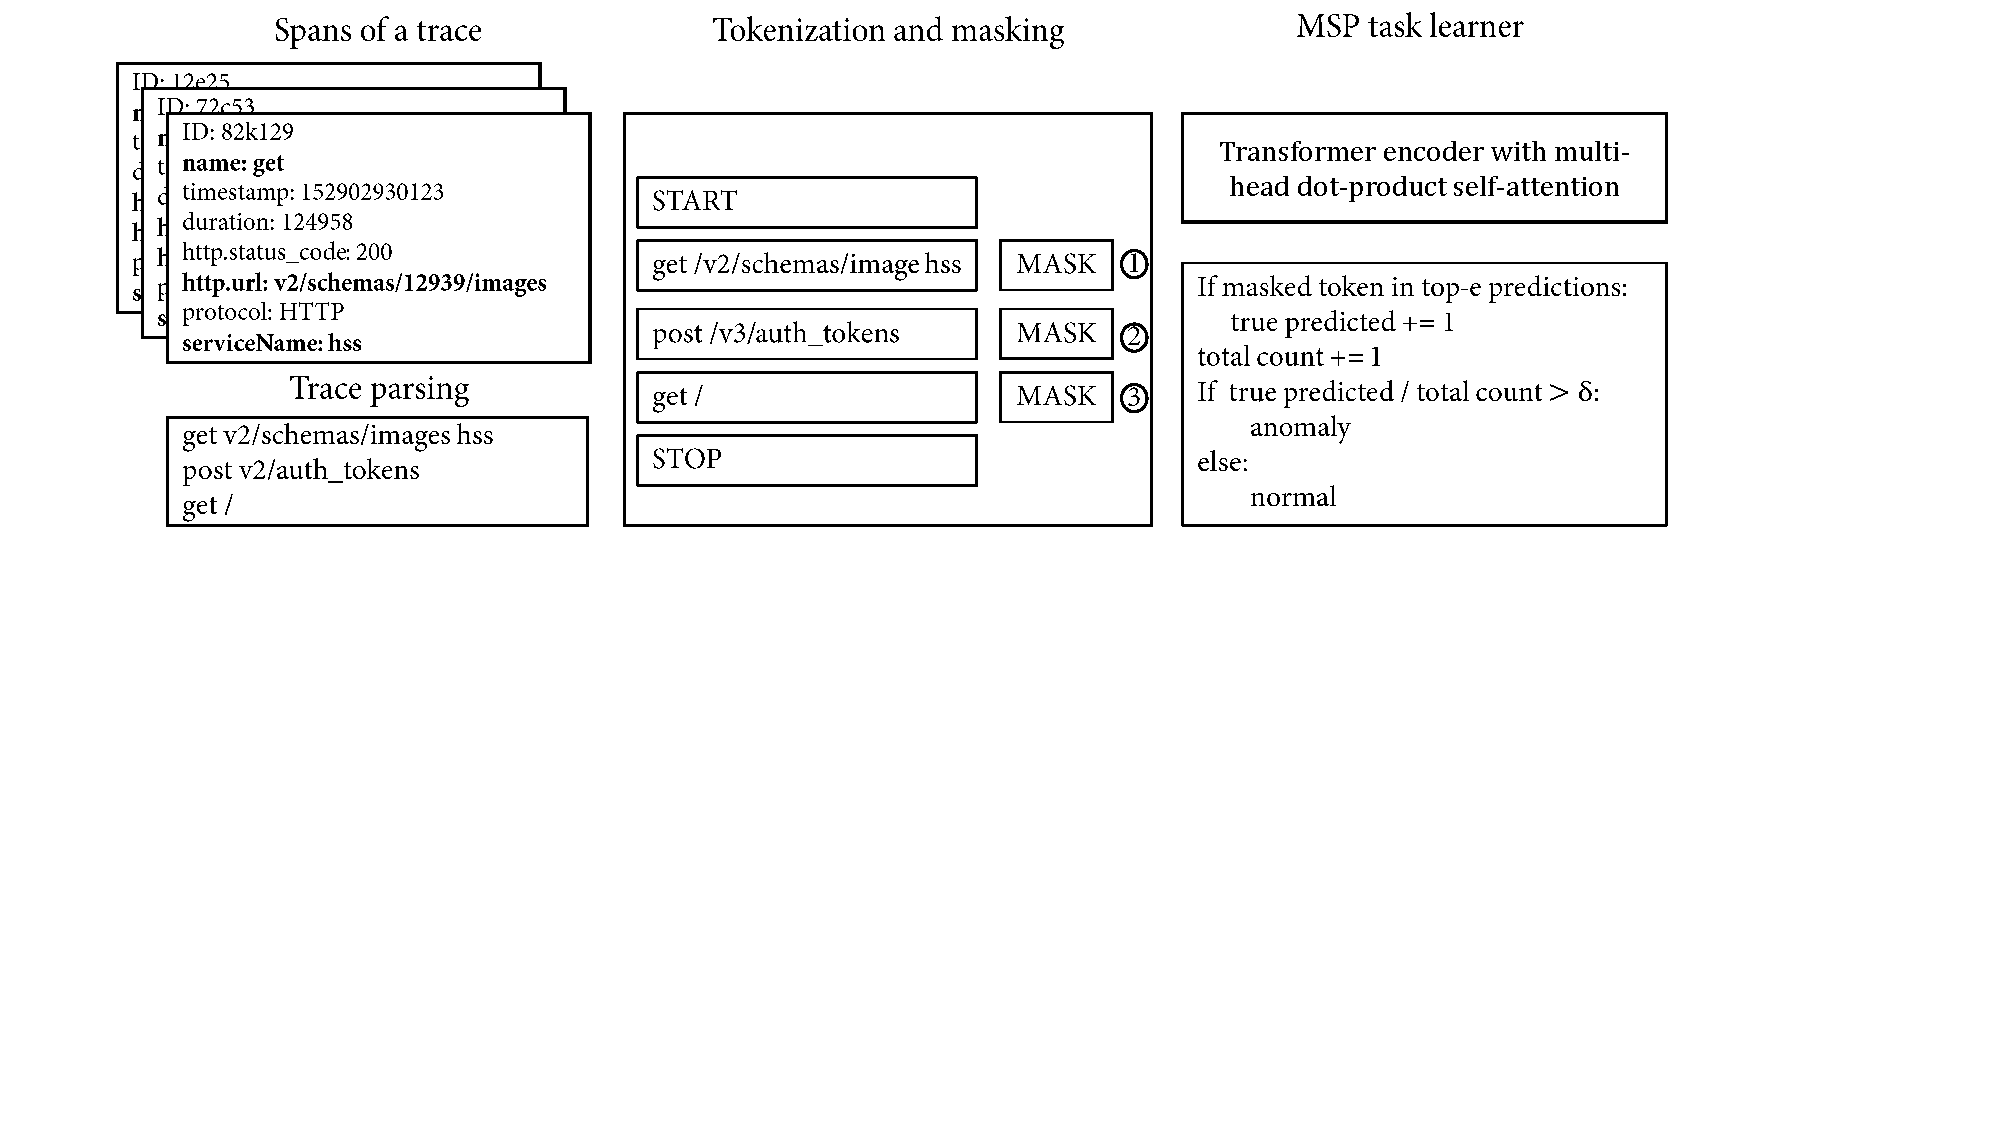
\includegraphics[width=1.0\textwidth]{gfx/chap6/overviewtracy.pdf}}
\caption{Overview of Tracy.}
\label{fig:tracyarchitecture}
\end{figure}

To train a contextual representation of the spans and trace from both forward and backward contexts, in Tracy, we mask a percentage of the input spans at random, and then predict the masked tokens (see Figure~\ref{fig:tracyarchitecture}). To this end, Tracy learns the likelihood of appearance of particular span with given context spans. We utilize this as a proxy task for anomaly detection, which we refer to as masked span prediction (MSP), similar to MLM in~\autoref{ch:logs:logparsing}. With such a learning task, we model the traces representing the normal behavior of the system. In the prediction phase, if a trace is normal, the success rate of correct prediction of the masked spans with given context spans will be high; otherwise, the success rate will be low, suggesting an anomalous trace. Thus, introducing a threshold on top of the success rate of correctly predicting the masked spans within the trace is utilized to decide whether the trace is anomalous or normal. 

To solve the MSP task, we use the transformer encoder neural network architecture. It is based on the attention learning concept, which, in the context of traces, relates the input spans to given target (masked span). The underlying learning mechanism (self-attention~\cite{vaswani2017attention}) enables the target to be selective on which spans are relevant. In the case of traces, this allows a sparse representation. It enables the trace to be represented with only the spans that are core and must appear in normal traces, minimizing the effects of the noisy spans. In other words, it builds abstract span representations that contain information for short and long interdependencies. Formulating the problem of trace anomaly detection as MSP enables to capture the complete end-to-end execution path among all involved components of the system. 


\begin{figure}[htbp]
\centerline{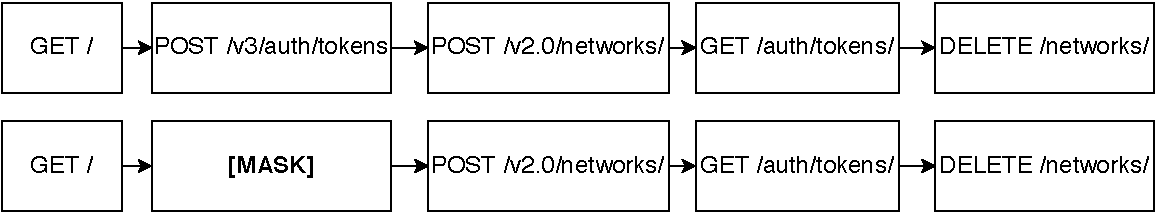
\includegraphics[width=1.0\textwidth]{gfx/chap6/exampleTracesMask.pdf}}
\caption{(Top) Example of \textit{network create and delete trace}. (Bottom) Example of the context of the \texttt{POST /v3/auth/tokens/} span used for the input of the self-attention mechanism. \textit{POST /v3/auth/tokens/} is denoted as masked span.}
\label{fig:exampletrace}
\end{figure}

The step after preprocessing is to perform masking. We illustrate the masking of an example trace in Figure~\ref{fig:exampletrace}. In the bottom line of the image, the \textit{POST /v3/auth/tokens/} span is replaced by the \texttt{[MASK]} span. A masked span in a trace can be any randomly chosen span that during the learning procedure is labeled with a special \texttt{[MASK]} span from the input. During the learning procedure, the true value of the masked token is used as a target and predicted by the remaining spans that construct the context (used as an input). This enables the masked span to "score" the relevance of the spans from the context for its prediction. With the span masking procedure, we produce training samples for every masked span. For example, if we mask two spans of a trace $T$, the masking module will produce two traces, each having one masked span. This enables one trace to be replicated multiple times and different contexts for the spans of traces from different workloads to be learned. Moreover, such masking of the spans that leads to various contexts for prediction of a span acts as a regularization technique to improve the robustness~\cite{devlin2018bert}. Intuitively, noisy spans that appear infrequently will be masked only few times, in contrast to spans that are frequent. Whenever a previously unseen normal trace from a known user request is presented to the method, according to the described property, the self-attention mechanism will be less sensitive to the changes that appear owing to noisy spans. Thus, the masking and self-attention mechanism enforce the model to focus on learning to attend core spans that appear in the trace.

After the masking procedure, the trace is modified to  
\begin{equation}
    T_{i}^{preprocessed}=([START], S_1^i, S_2^i, \texttt{[MASK]}, \dots, S_{T_{max\_len}}^i, [STOP]),
\end{equation}
and as such is utilized as an input to the neural network.

\begin{figure}[!t]
\centerline{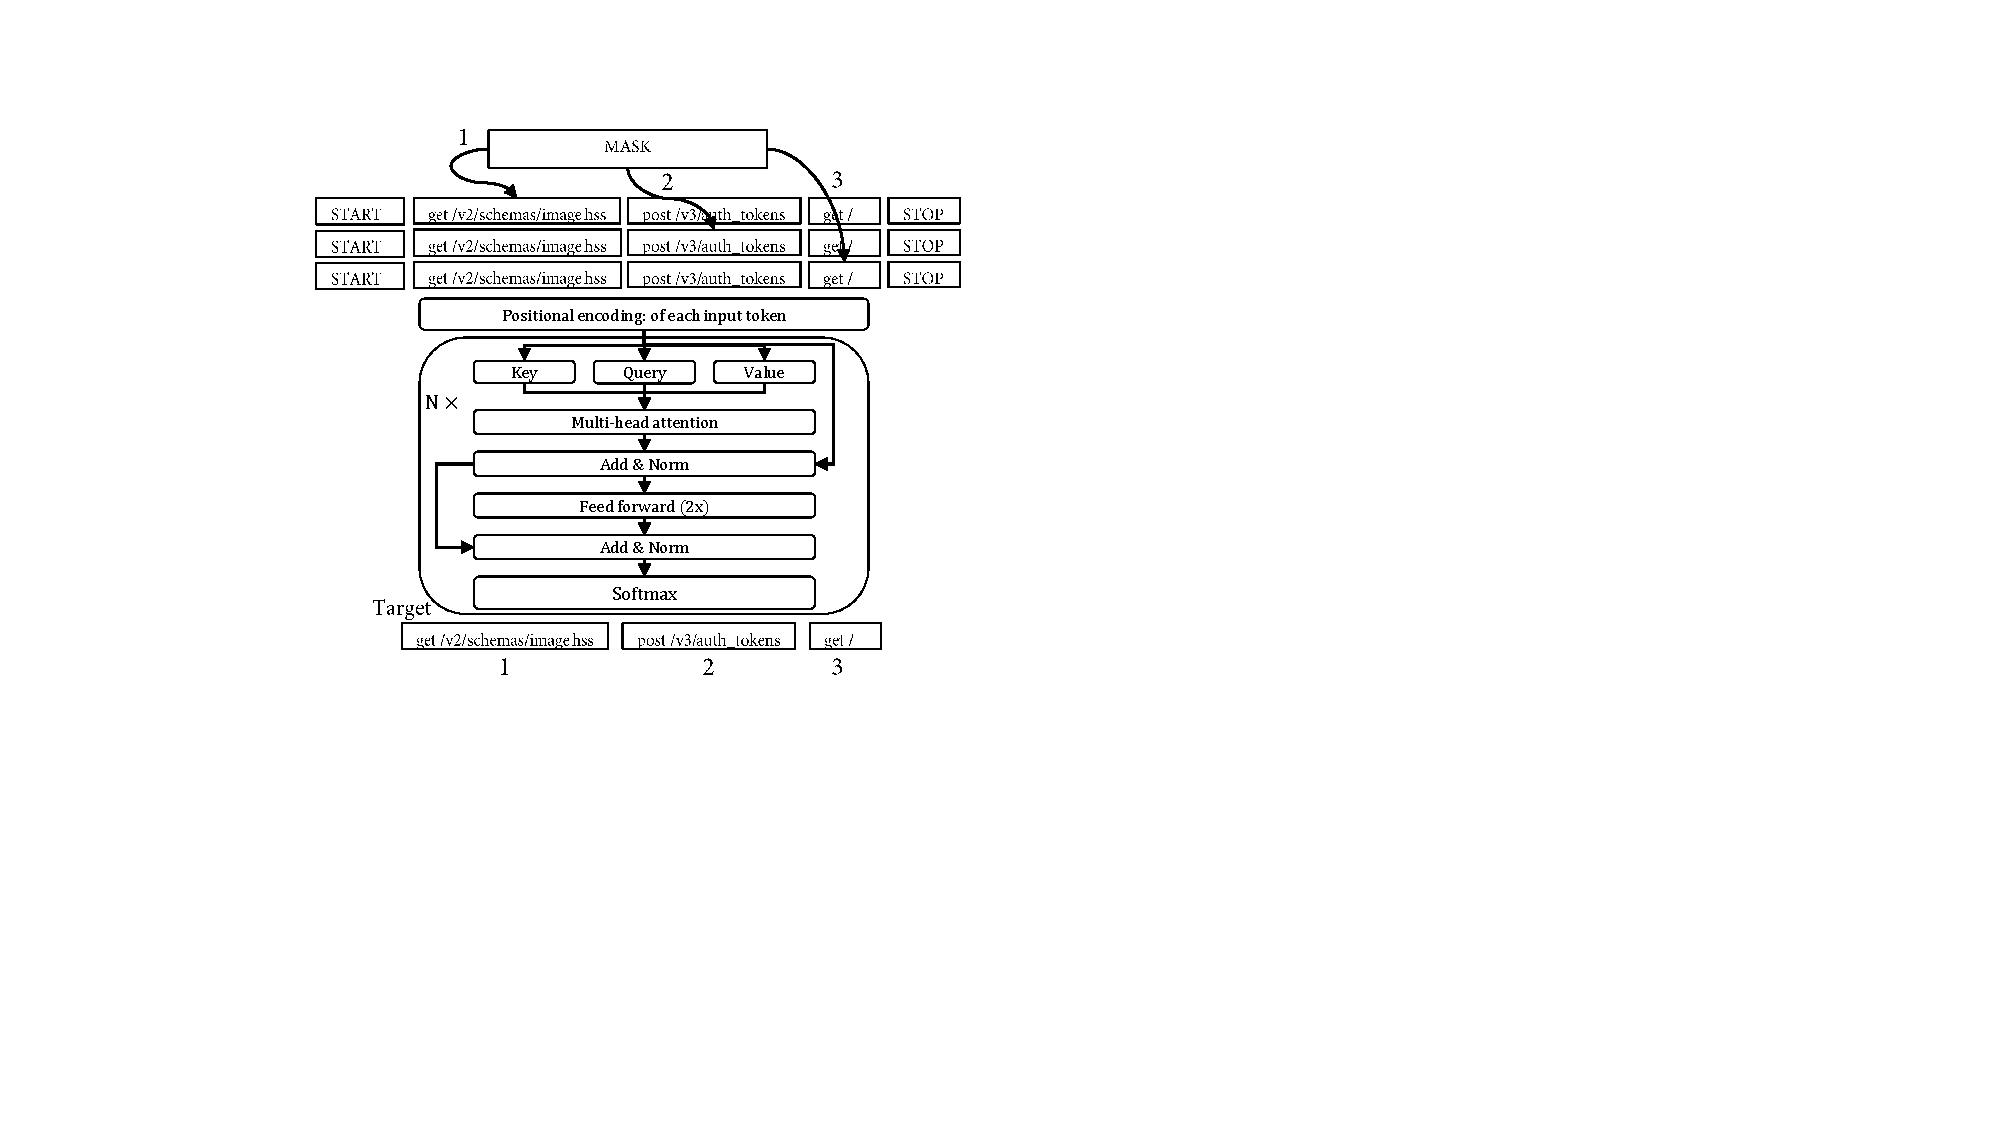
\includegraphics[width=1.0\textwidth]{gfx/chap6/tracymultihead.pdf}}
\caption{Neural network architecture used to solve the MSP task.}
\label{fig:msptracy}
\end{figure}

Figure~\ref{fig:msptracy} depicts the model's architecture. It is an encoder--decoder structure that maps the input spans in a vector format, learns higher-level abstract representations, and projects them to a probability distribution over the vocabulary of spans. The encoder uses a multi-head self-attention mechanism as a basic building block. 

The processed inputs are fed into the network. To preserve the sequential information, each span is encoded with an additional position value. Formally, this block calculates a vector that maintains the relative position of a span within a trace. Similar to the positional encoding in the log data (\autoref{ch:logs:logparsing}), the positional encoding block implements this by adding periodic functions (e.g., sine and cosine) to the vector representations of the spans in the trace.

The multi-head attention block is a neural network architecture, which implements the self-attention mechanism~\cite{vaswani2017attention}. It operates by projecting the input context for the masked span into various subspaces and aggregating them. Each projection is controlled by one of the $L$ heads of the multi-head attention. The multi-head block uses three vectors, key, query, and value, as an input. It uses the key and query of the current input representation to assign scores for the context spans from the trace to the current masked span. Intuitively, this part learns the influence of the context spans on the prediction of the masked spans. 
% As the multi-head attention block was already described in detail in \autoref{ch:logs}, we skip additional mathematical formalities.

The next part of the network consists of two feed-forward layers. They provide a richer representation of the underlying output of the multi-head attention mechanism. The outputs are fed through a one-layer network with softmax at the end, which serves as a decoder. The softmax is used as a function to generate probabilities over the whole dictionary of spans. These probabilities suggest the likeliness of the current masked span to be associated with a symbol within the vocabulary of symbols conditioned on the context. 

\subsection{Detecting anomalies}
The MSP is a proxy task for anomaly detection. As a standalone task, it cannot be used for anomaly detection. To this end, we introduce an additional postprocessing of the predictions of the MSP model to detect anomalies. The output from the MSP for a particular trace and masked span is an ordered list of predictions as possible spans for the masked position in the trace. The lists are ordered according to their relevance (probability) to be the particular masked span. During the anomaly detection, each of the ordered lists on the particular position in the trace is analyzed in the following manner. If the observed value on a particular position of the trace is not in the first $top-k$ elements of the list generated by the MSP task module for that position, we consider the span as incorrect. We count the errors for each trace and divide their number by the trace length forming the ratio of misclassified examples or span error rate per trace. The span error rate serves as an anomaly score. If a model leads to many mistakes, the anomalous score is higher, and thus the trace is anomalous. Setting a decision threshold on the anomaly score can be used to decide whether the trace is normal or anomalous. The span error rate is another key characteristic of the method that addresses the noise in the traces. In the following section, we empirically demonstrate the validity of these claims.

\newpage

\section{Evaluation}
In this section, we describe the data utilized for the evaluation. We describe the learning scenarios (LSs) used to evaluate the performance of our method and present the results. We investigate the differences in the attention scores between the normal and anomalous traces and their utilization to infer characteristic differences between the normal and anomalous traces.

\subsection{Experimental data}
We evaluated the presented method on two separate datasets, a dataset from a planet-scale industry system (referred to as production data) and dataset generated from our testbed deployment. The experiments were performed on a GPU NVIDIA 1660Ti (6GB) and CPU Intel(R) Core(TM) i7-9750H CPU at 2.60 GHz.

\textbf{OpenStack~\cite{ShrivastwaOpenstack} testbed.} It is based on a microservice architecture, running in a dockerized environment Kolla-Ansible~\cite{kollaansible}. OpenStack was deployed on four compute and one control nodes. 

The normal and anomalous data are generated by the execution of three workloads. (1) \textit{Create and delete server} uses a task from Rally~\cite{rally} to create and delete a VM. The fault is injected in a compute node, which restarts the API container that runs on the compute nodes. (2) \textit{Create and delete image} uses the \textit{glance} project of OpenStack to create and delete an image. The faults are injected by restarting the glance-API, which runs on the controller node. (3) \textit{Create and delete network} is a an operation that provides a network interface. The anomaly is injected by disruption of one of the neutron services (e.g., neutron metadata agent, neutron server) during the creation of a network.

To represent a scenario close to the real world, the workloads are executed concurrently. As some operations are faster than others (e.g, we need more time to boot a machine than to create a network), the workloads are performed with different numbers of iterations. 2000, 3000, and 6000 iterations for create and delete server, create and delete image, and create and delete network were carried out, respectively. The injections of the faults were carried out at every 250 iterations for \textit{create and delete server} and \textit{create and delete image} and every 500 iterations for \textit{create and delete network}. After the execution of the sequence of workloads, reports for the conducted experiments are generated. The reports contain details for the successful execution of the workload. They are used to induce the ground truth label for a particular user request. This is needed to separate the normal from anomalous traces to perform the evaluation.

\textbf{Production data}. Even in small controlled experimental setups, the noise is high and the traces change over time. This already poses challenges for the anomaly detection. However, testing the approach on large-scale production cloud data is required to show the viability of the approach. It covers traces from the creation of a VM upon request from the user. A characteristic property of production traces is their significantly larger length than those of the experimental testbed. The production data available in this experiment contained 200 traces with different lengths. 

\begin{figure}[htbp]
\centering
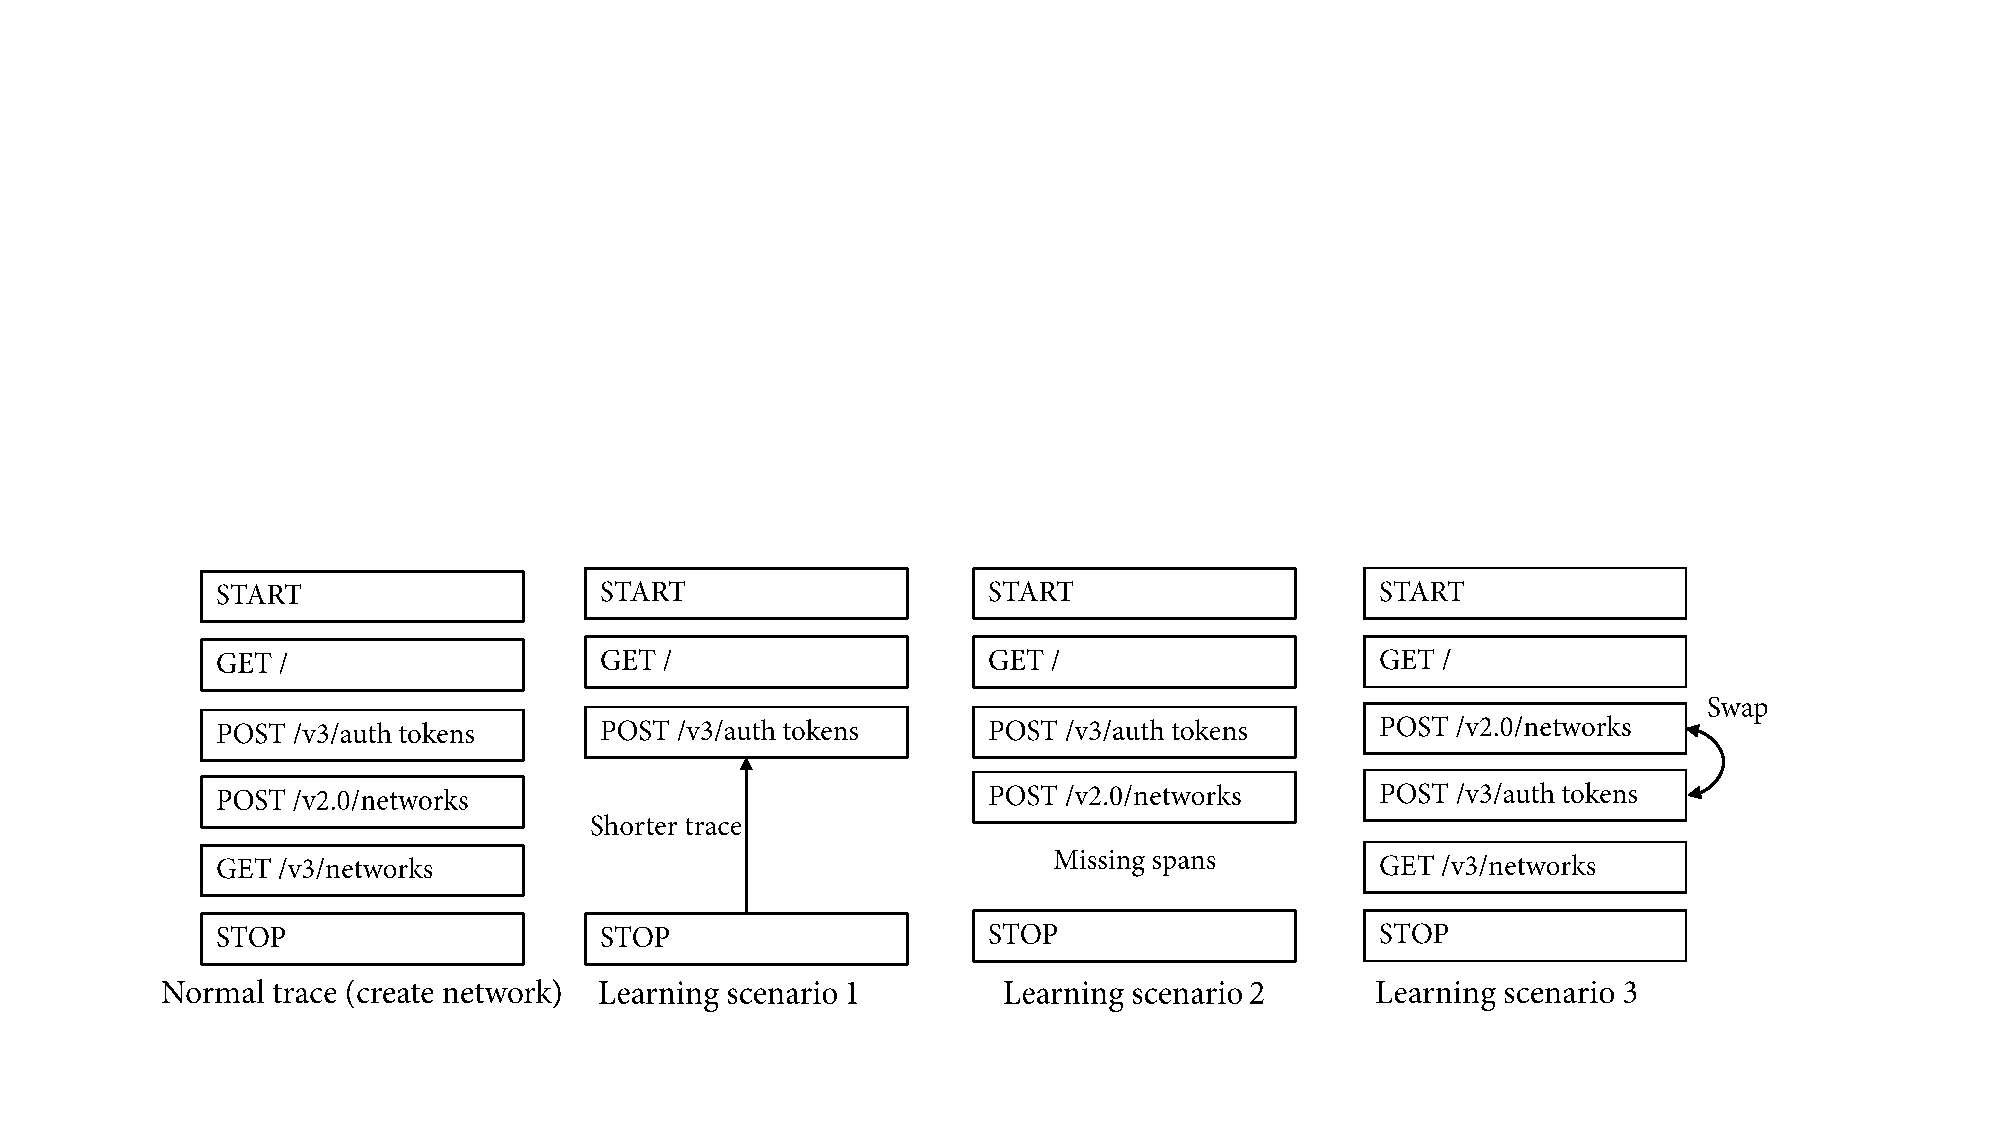
\includegraphics[width=1.0\textwidth]{gfx/chap7/traceanomalyinjections.pdf}
\caption{Anomaly injection scenarios in trace data.}
\label{fig:traceanomalyinjections}
\end{figure}


\subsection{Learning scenarios}
To evaluate and compare the performances and robustness of the proposed attention method and state of the art in anomaly detection from tracing data, we consider three LSs (see Figure~\ref{fig:traceanomalyinjections}). To test the ability of Tracy to preserve the global and local properties within the traces, we grouped our experiments into three groups (short, long, and combined (short and long) traces). The definition of these categories is data-driven, which implies that short traces are considered those that are concentrated around the lower values of the trace lengths ($\leq median$). The remaining traces belong to the category of long traces. 

\textbf{Real anomalies (LS1)}. In this LS, in the test set, the anomalies generated by the deployed testbed were used. The aim of this scenario is to evaluate the performances of the methods for anomaly detection from tracing data in the presence of anomalies generated by the system.

\textbf{Artificial anomalies (LS2)}. The anomalies in the traces are usually reflected by shortened traces, according to the procedure that generates the anomalies. Restarting a service interrupts the trace at particular span. The anomalies can be injected at every span in the trace as every span represents a service that can be malfunctioning. To evaluate the generalization and robustness of the method scaling to different types of anomaly, a set of artificial anomaly tests is created. The creation of this set is carried out in a manner that $L$ traces from the normal test set are selected at random. The selected traces are truncated at random position. These traces are labeled as anomalous and are joined with the remaining normal traces to create the test set.  


\textbf{Span permutation (LS3).} Owing to various reasons (e.g., an increased number of user requests or caching), some of the traces may have different orders of appearance of the spans, but still complete the whole operation, which implies that the trace is normal. In this LS, the test data are constructed as follows. First, a random selection of a normal trace is carried out. Second, a random span is permuted with its right neighbour, if existing. Third, this procedure is repeated for $L$ randomly selected traces composing the test set. In the test set, only normal traces exist.

We selected the best parameter configuration in LS1 and used it to evaluate the method in all LSs, LS1, LS2, and LS3. This enables to directly evaluate the changes in the performances of the methods to novel anomalies and random permutation in the neighbours, which reflects the ability of the method to handle traces with noise. To demonstrate the independence of the performance of the method on the position of the injected anomaly, we carry out an additional robustness test. During this test, 500 randomly selected traces among the normal traces are sampled. In each trace at each position, one of the spans is replaced by a randomly chosen span, while treating the changed trace as an anomaly. The experiments are repeated five times to obtain estimates for the expected performance score and its confidence intervals. 

\subsection{Baselines}
We compare Logsy against two publicly available methods, (1) LSTM-based trace anomaly detection~\cite{nedelkoski2019anomalymultimodal}, proposed in our earlier study and explained previously, and (2) TraceAnomaly~\cite{liu2020unsupervised}, a state-of-the-art method based on deep Bayesian networks with posterior flows. TraceAnomaly processes each trace as a whole to construct a service trace vector that encodes the invocation path. It then learns the overall normal trace patterns for a service during offline training. Lastly, in online anomaly detection, for each new trace, an anomaly score is computed, and accordingly traces with small anomaly scores are considered anomalous. As TraceAnomaly largely outperforms other more traditional methods such as string matches or finite state machines, we discard direct comparisons to these methods in our evaluation. The parameters of the LSTM-based method and TraceAnomaly are tuned to produce their best F1 scores.

\subsection{Results}
We present the results of the three LSs, including the precision, recall, and F1 score.

\begin{figure}[!t]
\centering
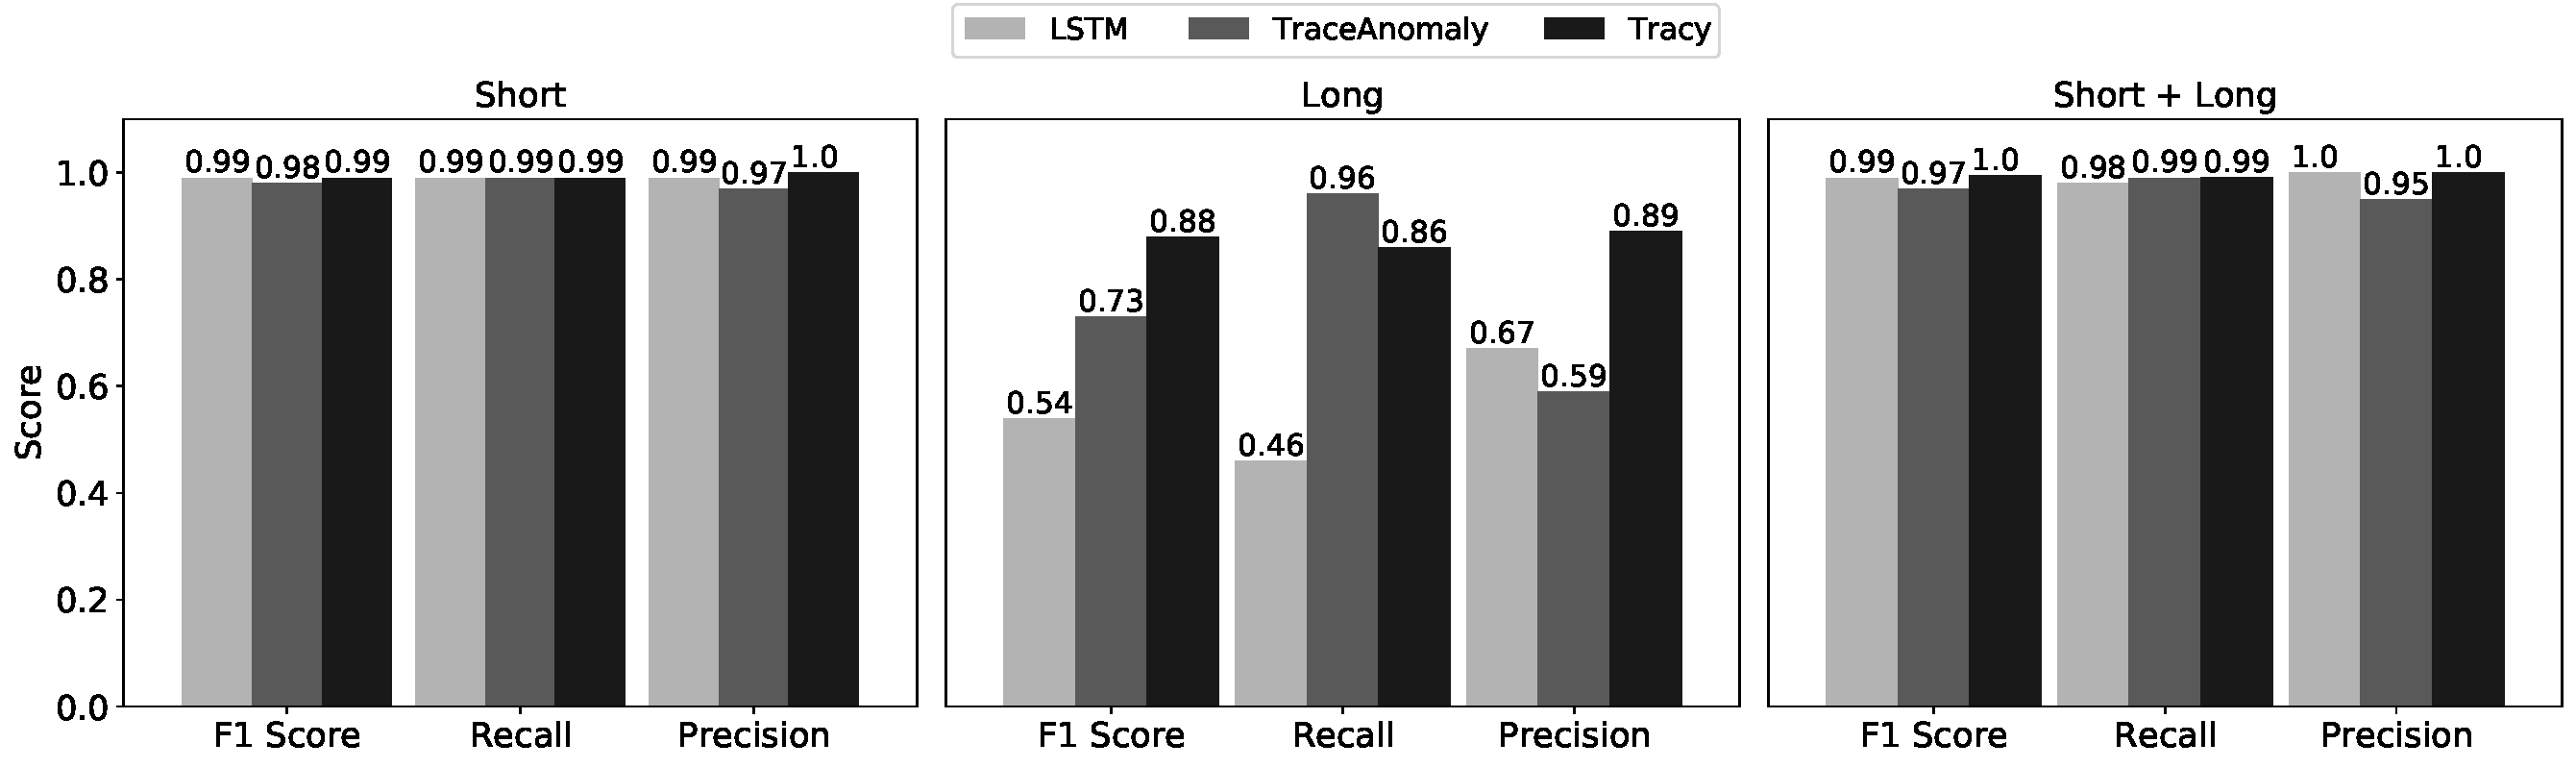
\includegraphics[width=1.0\textwidth]{gfx/chap6/ls1.pdf}
\caption{Results of the experiments for LS1.}
\label{fig:LS1}
\end{figure}

Figure~\ref{fig:LS1} shows the results of LS1 for the best-selected models from the optimization. When the long traces are considered, higher scores are obtained for the attention mechanism than those of the previous state-of-the-art methods, LSTM and TraceAnomaly, in all three cases. The attention mechanism can prioritize specific spans of the trace owing to the sparsity characteristic. Thus, the attention mechanism utilizes the most salient spans that form the trace. On the contrary, the LSTM-based method focuses on local properties of a trace owing to the autoregressive assumption. TraceAnomaly leads to problems in noise handling (e.g., changes in few spans), responsible for most false predictions. The comparable performances on the short traces are obtained as all methods utilize the locality in the traces. The largest advantage of Tracy over the state-of-the-art methods originates from the log traces. The performance of Tracy remains high even when traces are long. The precision for long traces outperforms the baselines by 0.3 owing to the reduction in number of false positive predictions. The good performance on the combination of the long and short traces for all methods (F1 above 0.9) is attributed to the imbalance dataset, where the number of short traces is considerably larger.

\begin{figure}[!t]
\centering
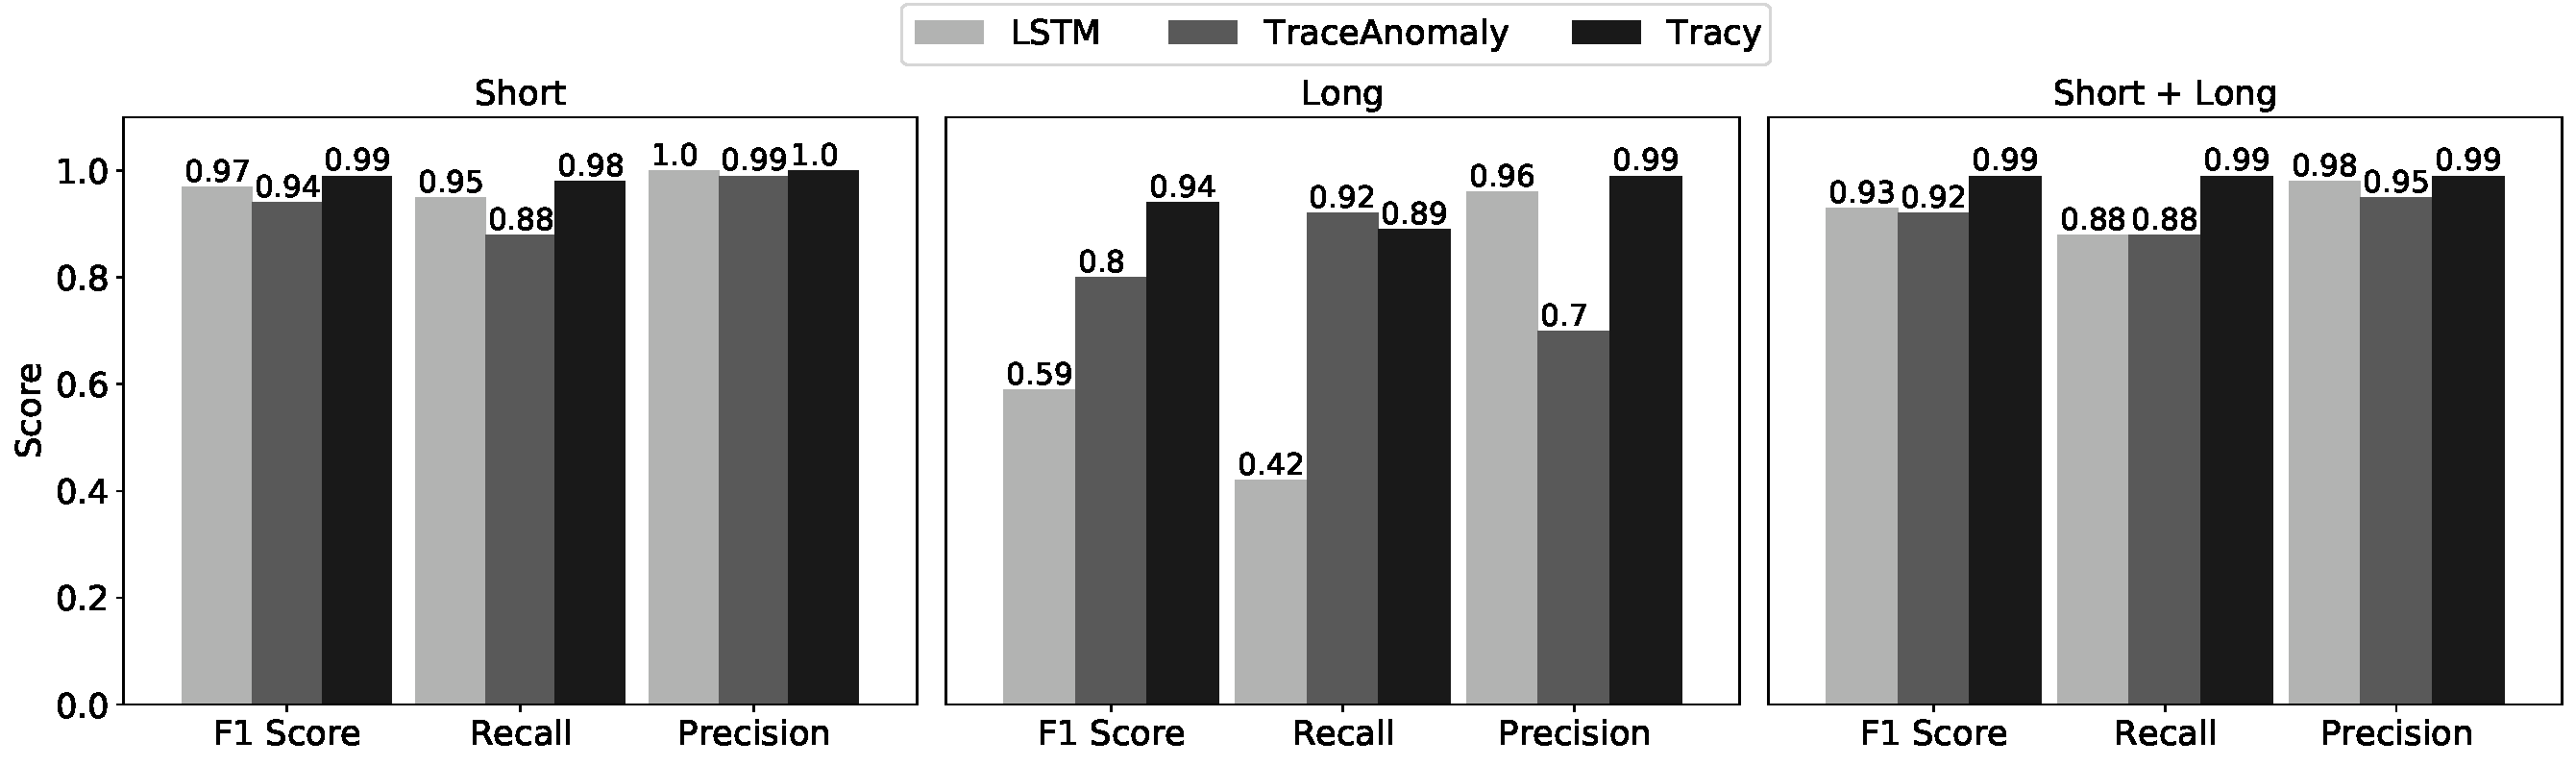
\includegraphics[width=1.0\textwidth]{gfx/chap6/ls2.pdf}
\caption{Results of the experiments for LS2.}
\label{fig:LS2}
\end{figure}

Figure~\ref{fig:LS2} shows the results of LS2. We observe a notable decrease in the recall for both small and long traces in LSTM and TraceAnomaly. This implies that, in this scenario, the baselines tend to produce an increased number of false negatives. This can be explained as the anomalous trace differs from the normal only in its length, owing to the inability of the methods to extract global patterns from the trace. The methods exhibit good performances for short traces and lower performances for longer traces. Long traces are more common in large distributed systems as they contain hundreds of services~\cite{nedelkoski2019anomaly}. Executing one operation in a microservice architecture includes invoking multiple services not necessarily only HTTP calls for the communication between the services. Hence, the ability to handle long traces is imperative for applicability in tracing data from real-world systems. 


\begin{figure}[!t]
\centering
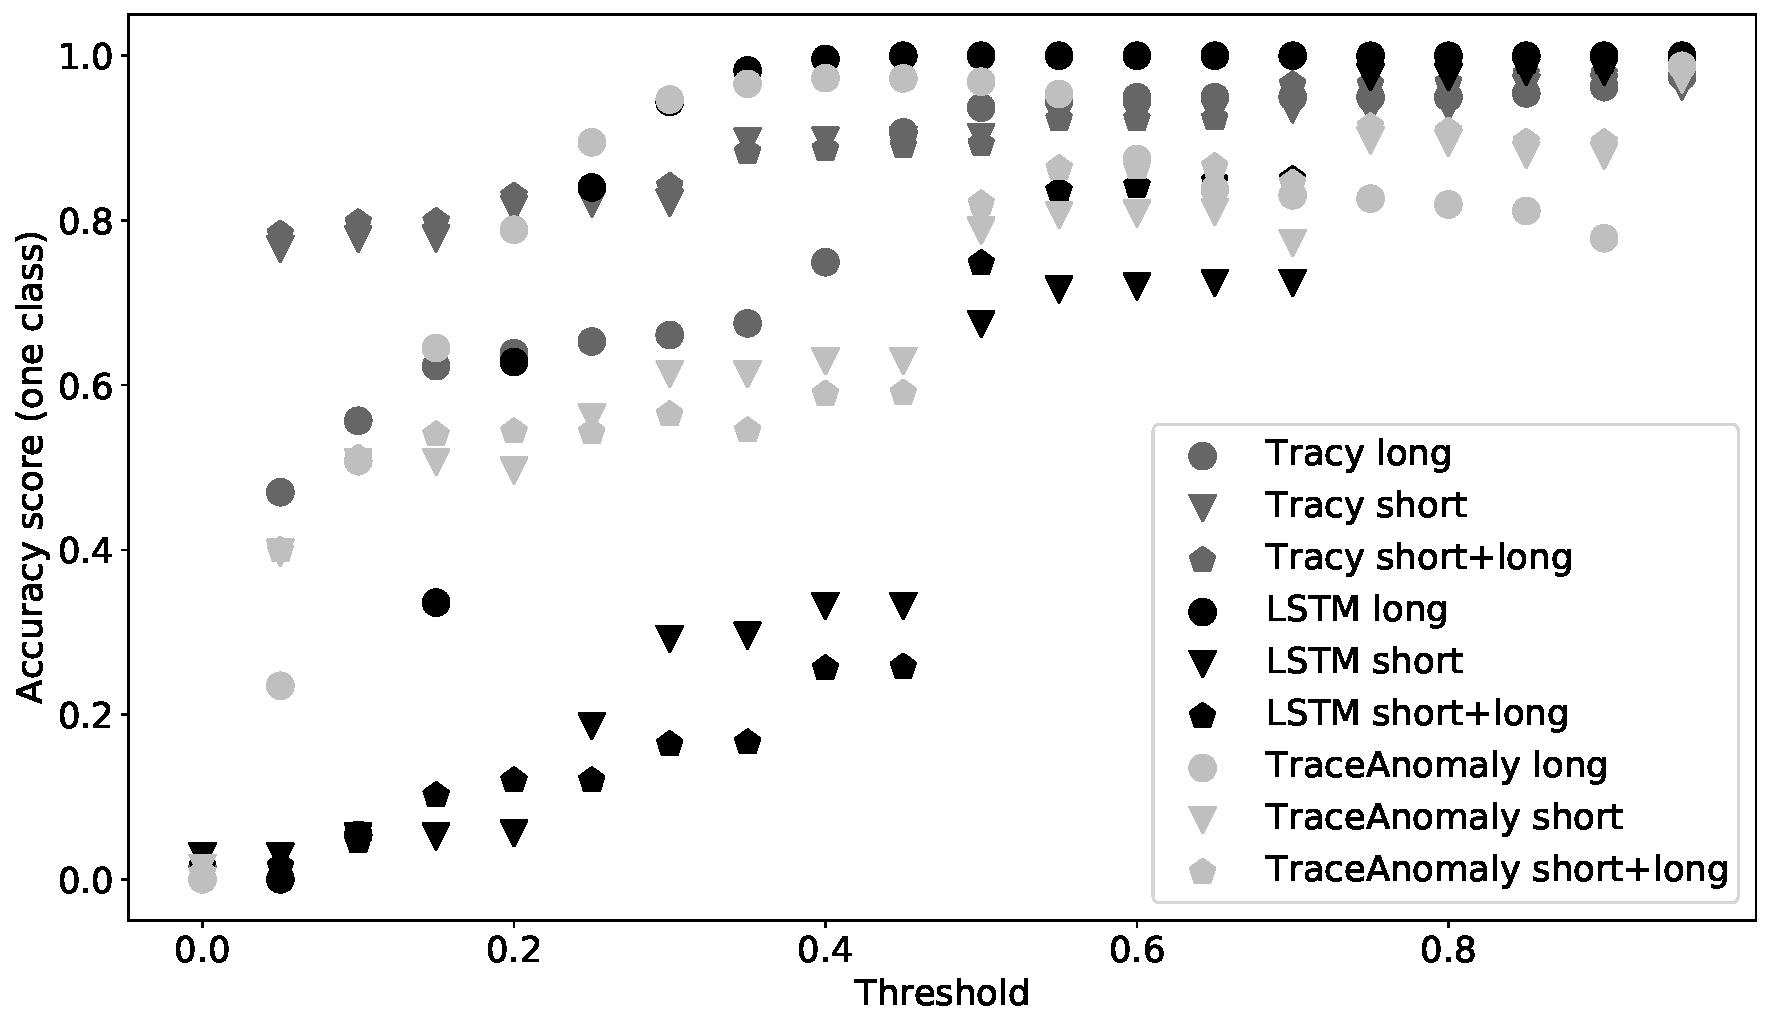
\includegraphics[width=1.0\columnwidth]{gfx/chap6/sensitivity_analysis.pdf}
\caption{Sensitivity analysis of Tracy vs. LSTM.}
\label{fig:3}
\end{figure}

\begin{figure*}[!t]
\centering
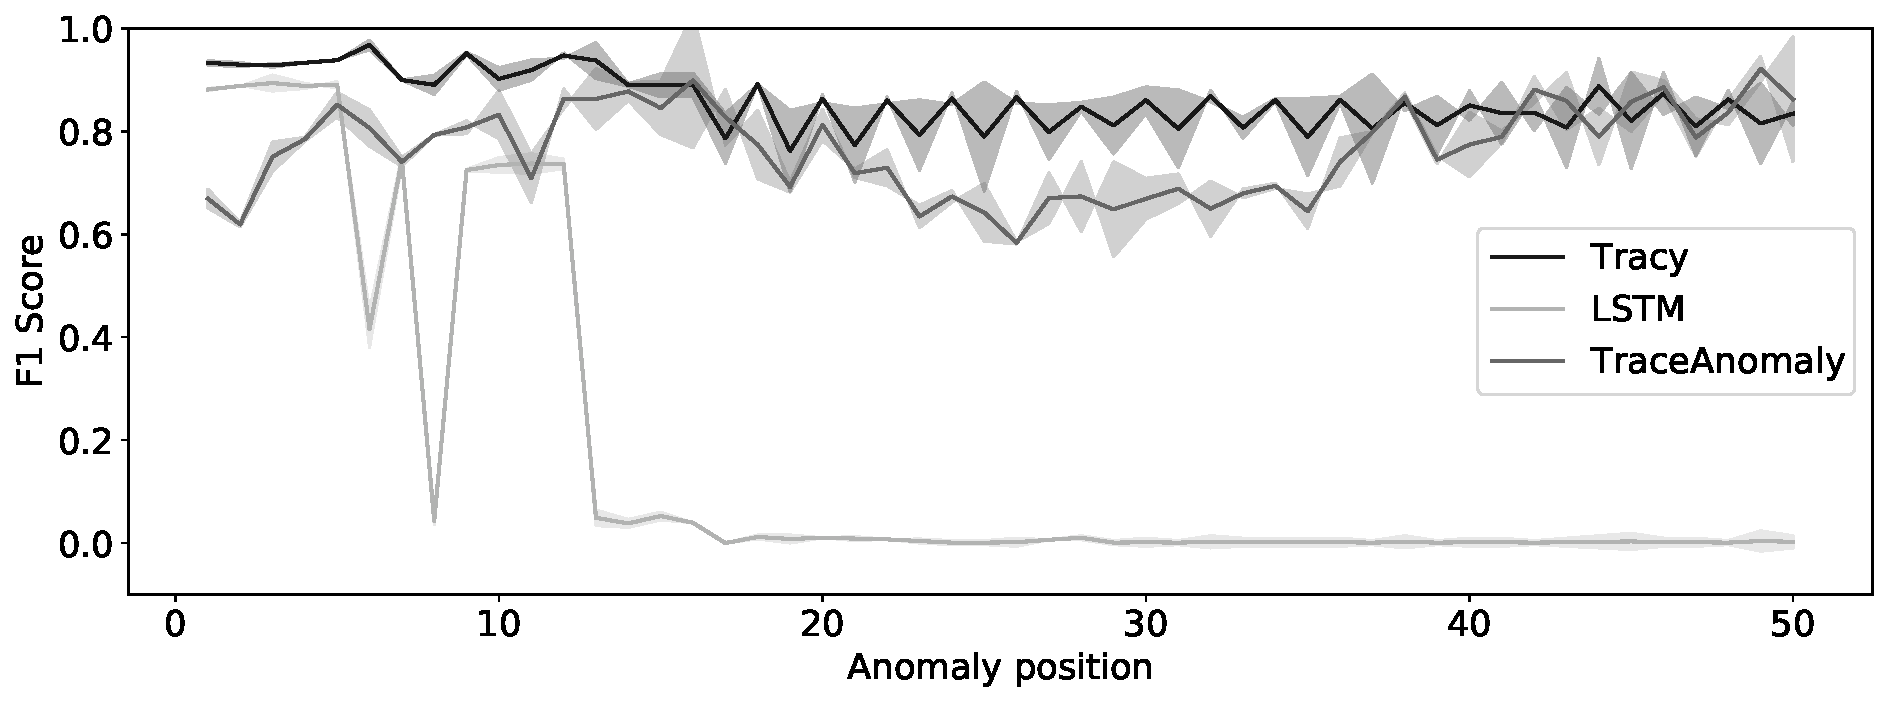
\includegraphics[width=1.0\textwidth]{gfx/chap6/positiontracy.pdf}
\caption{Performance score estimates with respect to the position of the injected anomaly. The solid line represents the mean value of the F1 score, while the shaded region is the confidence interval of one standard deviation.}
\label{fig:8}
\end{figure*}


LS3 evaluates the generalization ability of the method. Figure~\ref{fig:3} shows the results of \textit{LS3}. As it is a one-class prediction scenario, only the accuracy of correctly predicting the normal iterations is presented. This LS can be interpreted as testing the ability of the method to correctly predict novel normal traces that occur owing to the noise. The attention method is more robust than TraceAnomaly and LSTM. The cases of wrong classification in Tracy are mostly due to swapping of one of the "core" spans in the trace. Thus, the attention method cannot correctly predict the masked span. Nevertheless, on average, across all traces, the number of core spans for given trace is small, and thus the presented method exhibits a better score. LSTM and TraceAnomaly detect almost every change, which limits their noise robustness. However, TraceAnomaly has a higher noise tolerance than that of LSTM, achieving higher scores. 

To further evaluate the robustness of Tracy, in Figure~\ref{fig:8}, we show the F1-score with respect to the position of the injected anomaly. For the short traces (until 12 spans), the performances of the attention and LSTM-based methods are high and they are robust regarding the position of the inserted change. However, for long traces, a higher sensitivity of the LSTM-based method to small local changes within the trace is observed. This leads to a lower performance. These results show that the position of inserting a swap does not influence the performance of Tracy. The larger variance observed in the figure for the long trances is attributed to the small number of long traces in the training data. TraceAnomaly exhibits comparable performances to those of Tracy, as it also utilizes the global trace information.



\begin{table}[!t]
\centering
   \caption{Results for the production data from a global service provider.}

   \label{tab:1}
   \begin{tabular}{lrrrr}
     \toprule
     Dataset & Accuracy & Precision & Recall & F1  \\
     \midrule
     Production data & 0.92 & 0.91 & 0.95 & 0.93    \\
     \bottomrule
   \end{tabular}
\end{table}

\tablename~\ref{tab:1} summarizes the results for the production data. The method evaluation was performed by a global service provider to reduce the evaluation bias. Therefore, the experiments for the baselines were not performed. Tracy exhibits a high F1 score of 0.93, consistent with the results of the testbed evaluation. It demonstrates the usability of the proposed method for long noisy traces from a production setting. The analysis of the missclassified traces showed only small changes toward the last spans. 

\begin{figure}[!b]
\centering
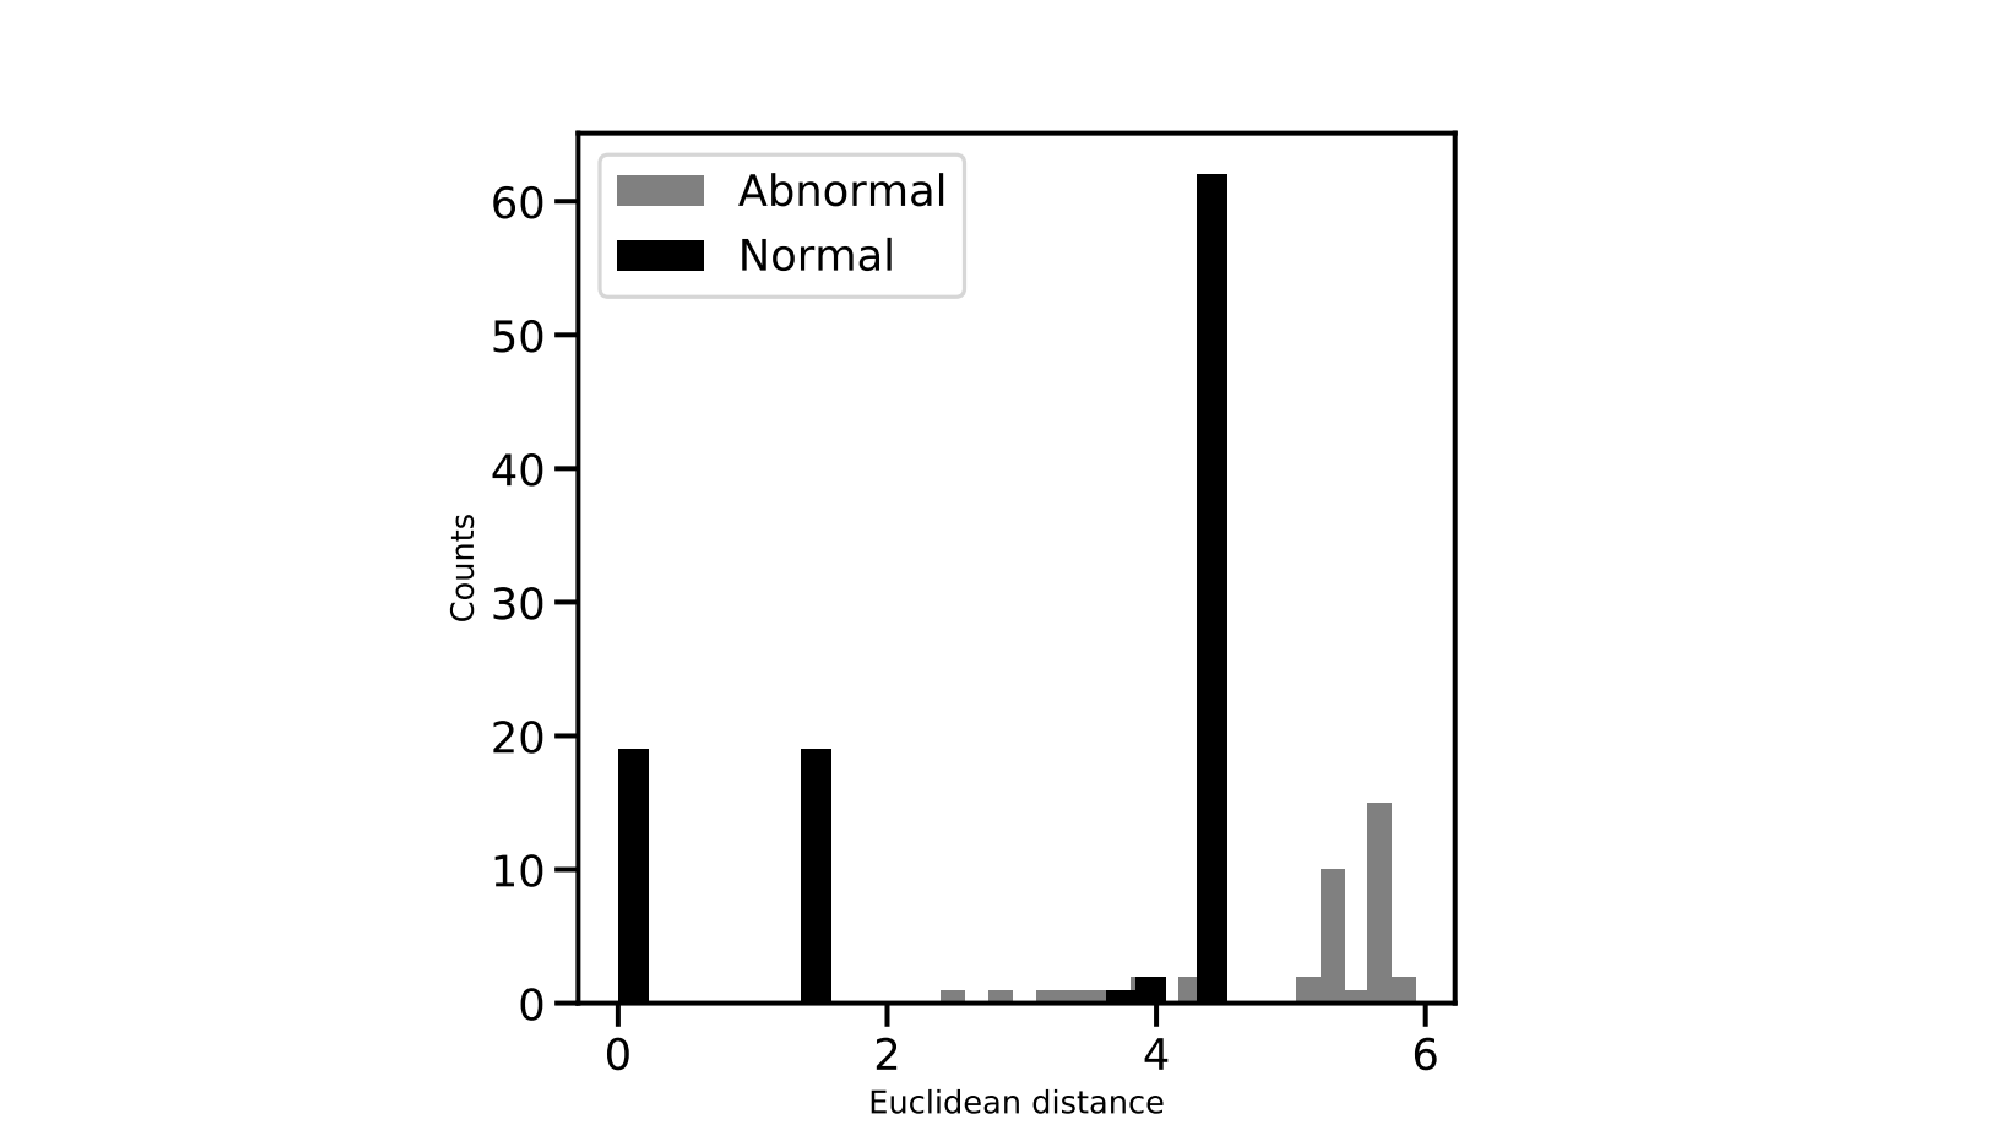
\includegraphics[width=0.55\columnwidth]{gfx/chap6/euc_distance.pdf}
\caption{Distributions of the distances of attention scores between the normal--normal (black) and normal--abnormal (red) traces.}
\label{fig:4}
\end{figure}


\subsection{Explanation of decisions}
The attention scores in the context of the MSP task are weights indicating the influence of each span of the trace on the prediction of the current masked span. These scores can be plotted in a heatmap and form a fingerprint. The spans that have the largest influence form a trace identifier. Figure~\ref{fig:4} shows the distribution of Euclidean distances of attention scores between normal traces (in black) and distribution of distances between the normal and abnormal traces (in red). A separation between the distributions can be observed. The distances between the normal and abnormal score matrices are larger. This suggests that observing the anomalous and normal self-attention scores can be utilized to indicate anomalous spans, which point out to anomalous services.

Figure~\ref{fig:5} shows the squared errors of the self-attention scores between normal and anomalous traces, where positions 2 and 4 are corrupted, respectively. An increased error at the particular position within the attention score matrix where the span was corrupted was observed. This indicates that the cross comparison between the normal and anomalous attention scores provides insights into the potential causes of the anomaly. In these examples, the deviations in the attention scores from the normal traces are emphasised at positions 2 and 4 of the trace. This shows that these positions are very unlikely to be occupied by the corrupted span. The operator can track the properties of this span and relate them to a potential cause.


\begin{figure}[!t]
\centering
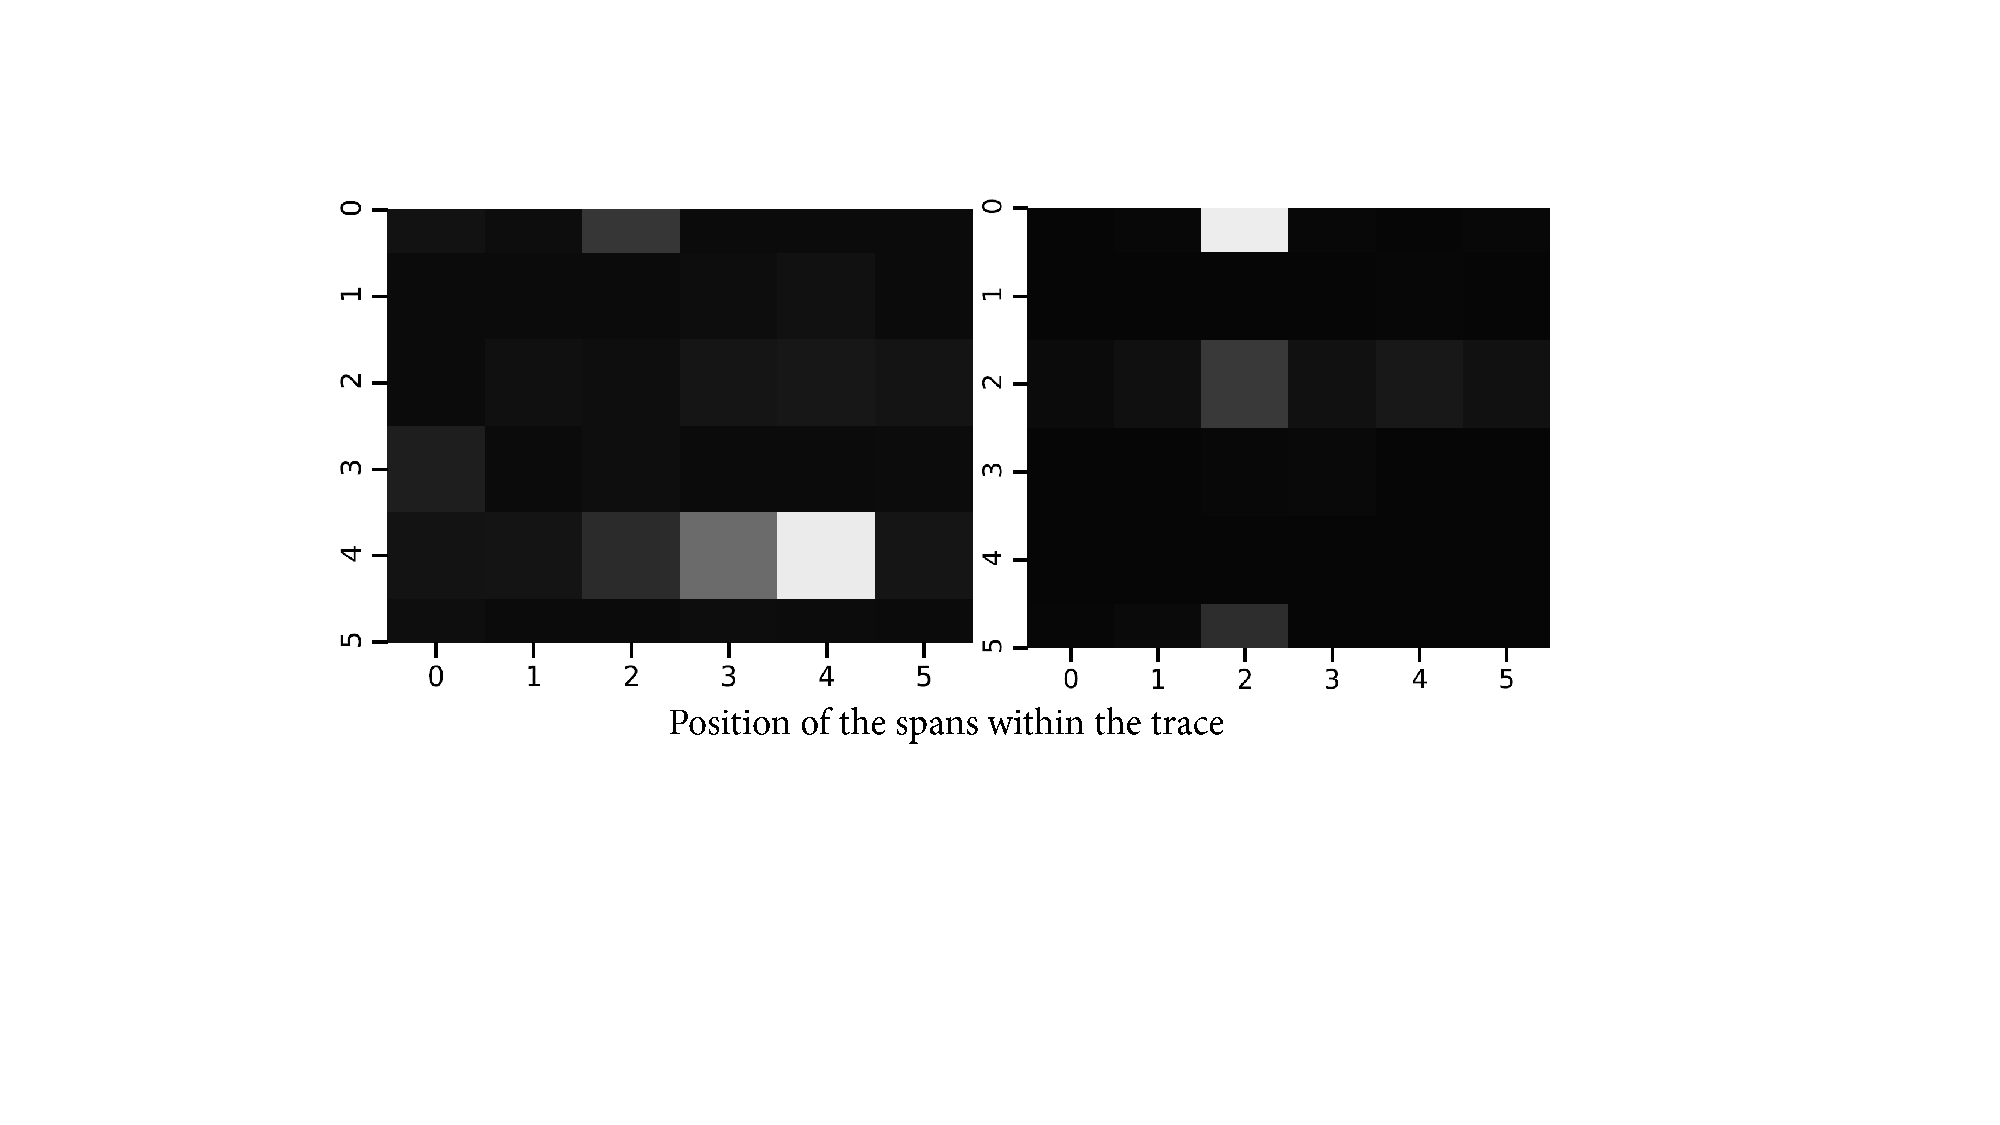
\includegraphics[width=1.0\columnwidth]{gfx/chap6/tracefingerprint.pdf}
\caption{Squared difference between the attention scores of normal and abnormal traces when an anomaly is injected at position 2 (left), 4 (right). The brighter color indicates larger scores.}
\label{fig:5}
\end{figure}


% \begin{figure}[!t]
% \centering
% \minipage{0.45\columnwidth}
%   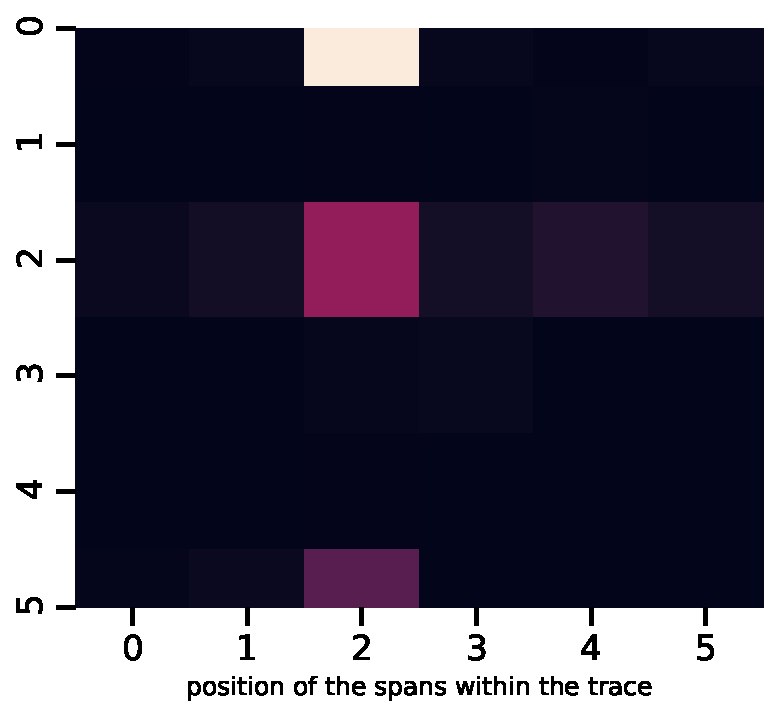
\includegraphics[width=1.0\columnwidth]{gfx/chap6/img.pdf}
%   \caption{Squared difference between the attention scores of normal and abnormal traces when an anomaly is injected at position 2. The brighter color indicates larger score values.}\label{fig:5}
% \endminipage\hfill
% \minipage{0.45\columnwidth}
%   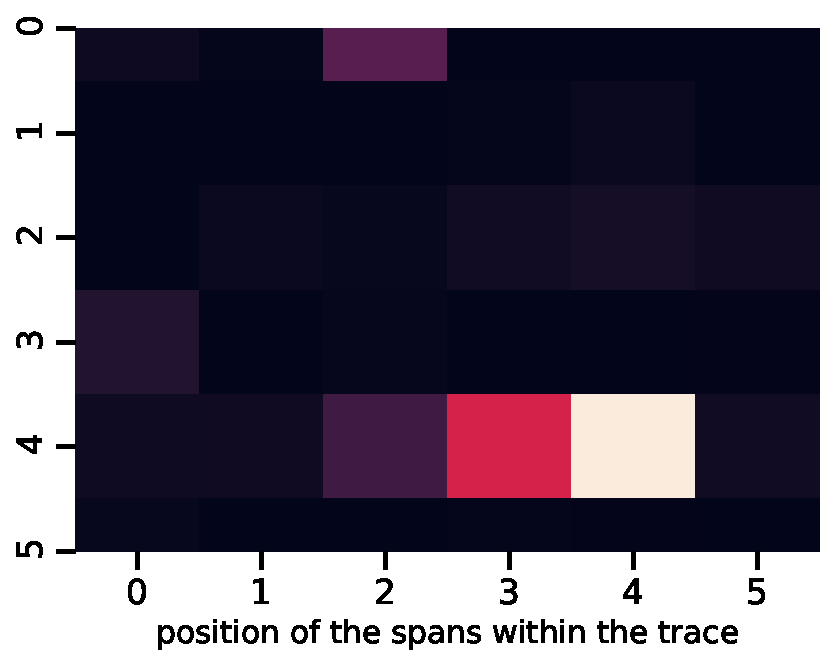
\includegraphics[width=1.0\columnwidth]{gfx/chap6/img2.pdf}
%   \caption{Squared difference between the attention scores of normal and abnormal traces for injection position 4.}\label{fig:6}
% \endminipage
% \end{figure}

\begin{table}[!t]
\centering
   \caption{Results of the correct localization of the inserted positional anomalies.}
   \label{tab:2}
   \begin{tabular}{lrrrrr}
     \toprule
     Position & 1 & 2 & 3 & 4 & 5 \\
     \midrule
     Correct prediction [\%] & 0.93 & 0.95 & 0.94 & 0.90 & 0.88    \\
     \bottomrule
   \end{tabular}
\end{table}


Furthermore, we replaced each position of the trace obtained by the execution of a \textit{create and delete} network request by random span. We computed the accuracy of correct span localization. Table~\ref{tab:2} summarizes the results. The attention scores can indicate the positional differences between normal and anomalous executions of a trace and thus locate the anomalous span.

\section{Related work}
Recently, extensive studies have been carried out on anomaly detection using tracing data. The straightforward approach for trace anomaly detection is based on string matching. For example, if a distributed system handles a user request by generating the sequence events/symbols $S_{1} = [M, N, O, Y, P]$, this sequence can be compared to a set of known sequences $S_{i}, \forall i\in \{0,\dots, N\}$, which represents the valid behavior of the system. If the sequence is found, the request is processed successfully. If sequence $S_{1}$ is not found, we can assume that a failure or anomaly occurred during the handling of the user request. However, the underlying volatility of the distributed system, as described in ~\autoref{ch:concepts:sec:anomalydetectionindistributedsoftwaresystems:subsec:trace}, makes the problem more complex than simple matching.

Three important requirements for anomaly detection from distributed traces exist. As described in \autoref{ch:concepts:sec:anomalydetectionindistributedsoftwaresystems:subsec:trace}, the methods should handle traces under the assumption of presence of noise, arbitrary lengths, and absence of labels.


\begin{figure}[htbp]
\centerline{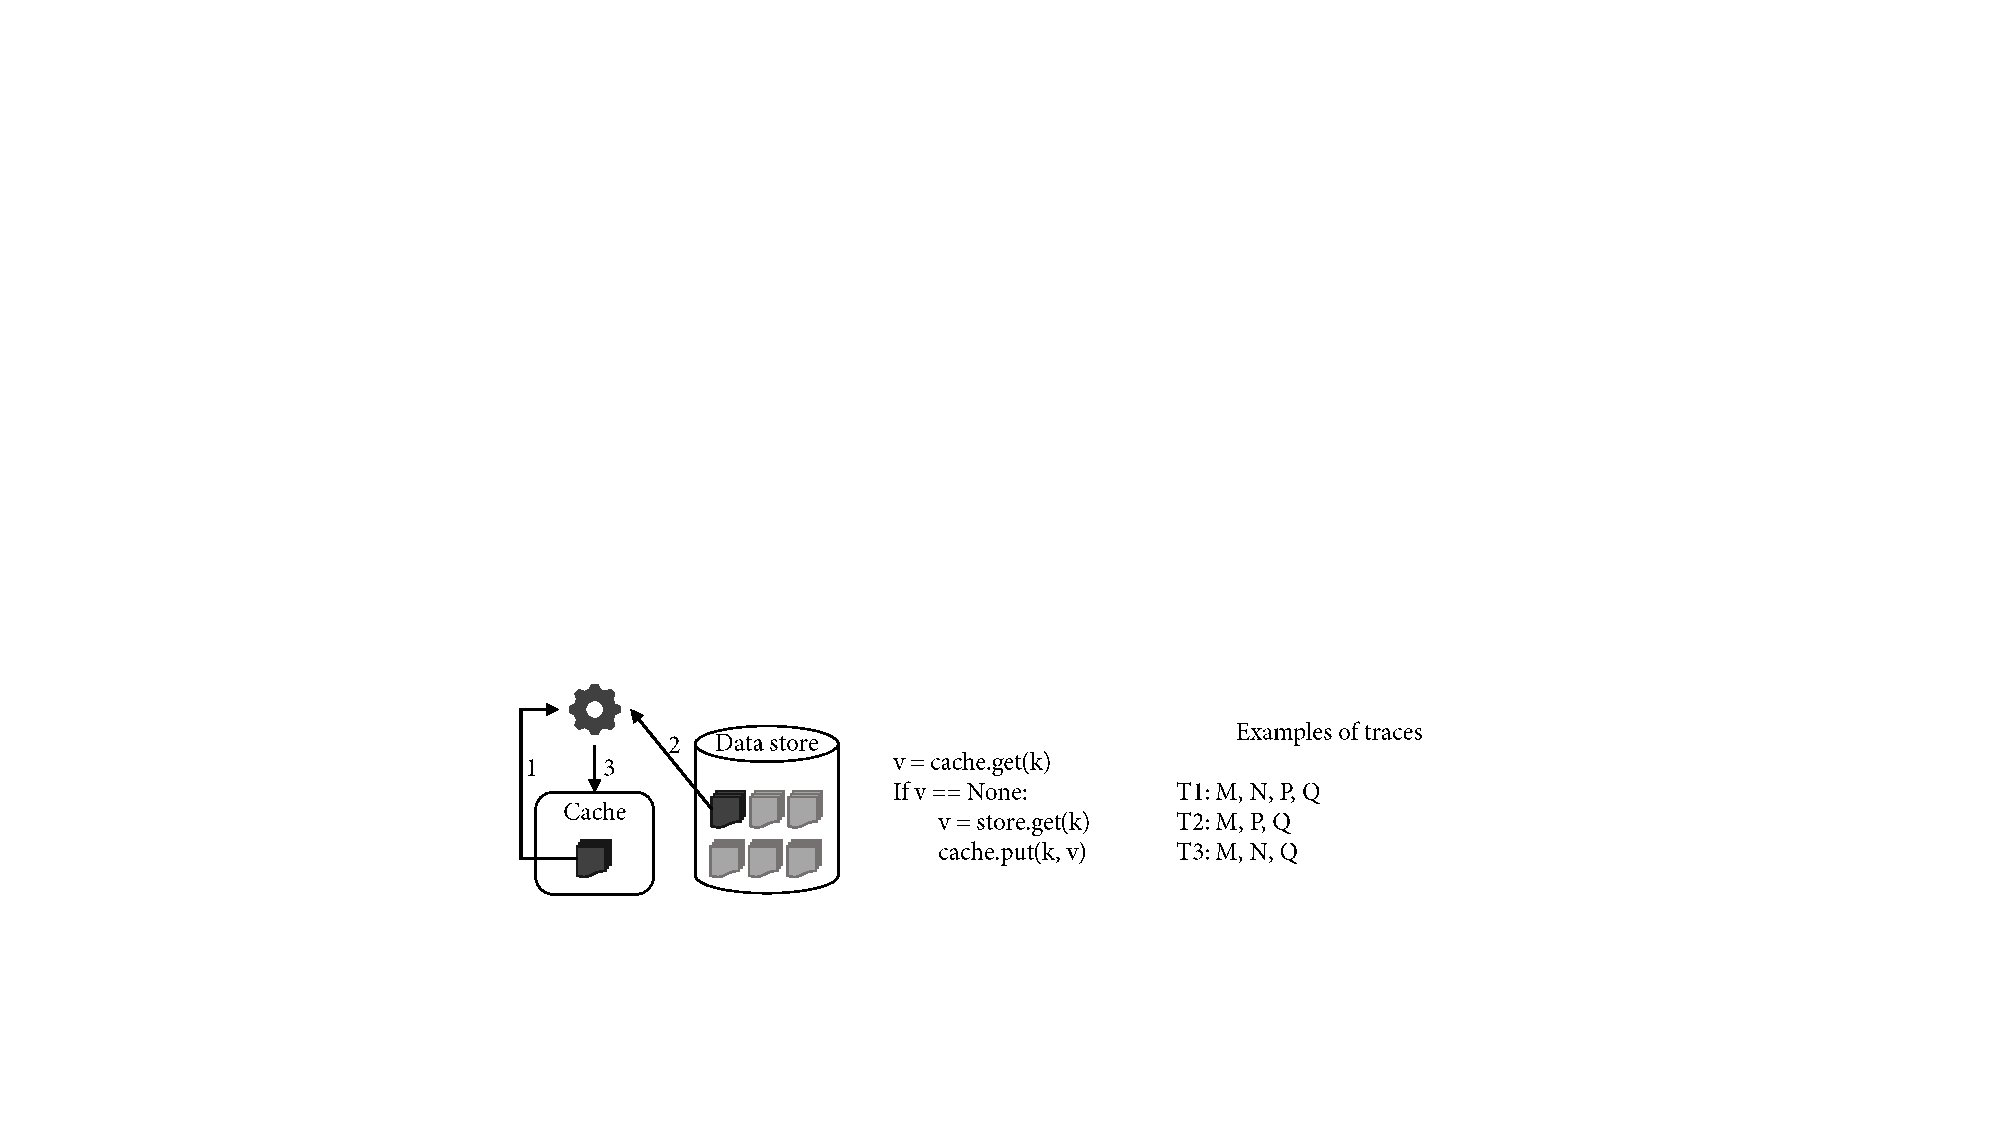
\includegraphics[width=1.0\textwidth]{gfx/chap7/cacheasidepattern.pdf}}
\caption{Caching and its effect on traces.}
\label{fig:cacheasidepattern}
\end{figure}

For example, noise can be caused by caching in distributed systems. It leads to suppression of symbols in traces as some instructions are not executed when the result is cached (see Figure~\ref{fig:cacheasidepattern}). Thus, a model can contain the following observed traces, [M, N, P, Q], [M, P, Q], and [M, N, Q]. When a new trace [M, Q] needs to be tested, it is intuitive that it is an anomaly as it was not seen in the past. Nonetheless, if we assume that the system under analysis can generate traces with noise, it is not obvious whether [M, Q] is an invalid trace or valid trace containing noise. The existing approaches, such as that in \cite{RepTrace}, use finite state machines (FSMs) to model the correct behaviors of systems. These approaches exhibit high performances when the traces do not contain noise. However, the introduction of noise scales the number of potential transitions exponentially. Thus, modeling noise using FSM-based approaches is not feasible as it will be possible to only model the already observed noise.

Approaches relying on LSTMs, e.g., those in our early study on an LSTM-based trace anomaly detection~\cite{nedelkoski2019anomalymultimodal,nedelkoski2019anomaly}, can process only traces up to a certain length of $k$. These approaches are referred to as autoregressive as they use previous symbols of a trace to predict the following symbol. For example, the developed techniques test the trace [M, N, P, Q, R, S] by predicting which symbol is after C according to a behavioural model, [M, N, P, Q, R]. If the prediction is correct (Q), the trace is classified as normal. Otherwise, it is anomalous. However, as traces become long, LSTMs are not capable of establishing a correlation between head symbols (M, N) and tail symbols (R, S). The first symbols of traces in a behaviour model are forgotten. This implies that the predicted symbol does not depend on all previous symbols. To address this limitation, approaches have been refined to use a sliding window with a size $< k$ over long traces. This strategy may improve the results but does not solve the problem that the symbols of a head trace are not considered by the prediction. 
The second drawback in these approaches is related to the production of more erroneous predictions because they observe only a fixed number of previous events to predict the upcoming event. Such models do not utilize the existing relation between distant spans in the trace. They learn the normal system behaviour from partial and limited data from previous events, which might affect the overall performance.

Recently, a new method denoted as TraceAnomaly~\cite{liu2020unsupervised} uses deep Bayesian networks to automatically learn the overall normal patterns of traces during periodic offline training. In online anomaly detection, a new trace with a small anomaly score (computed based on the learned normal pattern) is considered anomalous. TraceAnomaly, similarly to Tracy, utilizes global properties of the traces using variational inference. We identify the noise handling as the strongest drawback of TraceAnomaly owing to the lack of mechanism that prioritizes particular spans of the traces.

Lastly, methods from process-based anomaly detection~\cite{nolle2020process,PECCHIA2020105054,nolle2016unsupervised,nolle2018analyzing,nolle2019binet,imweber2015,xu2014weber,rehse2020} are related similarly. Weber et al.~\cite{imweber2015} describe two systems. The first, PODDiscovery, simplifies the creation of such an abstract process model (related to model of a trace) from operations logs. The proposed approach performs large amount of previously manual steps automatically, drastically reducing the time needed for obtaining the process model. Using the discovered model, the second system, PODViz, provides operators with the ability to visualize the current state of an operations process in near-real-time, and to replay a set of events to understand how the process context changed over time. There are several differences to the presented method--Tracy, namely, PODViz involves human interaction and obtains abstract representation from event logs into activities, which are related into a trace. On the other hand, Tracy performs end-to-end learning and detection of anomalies from the raw trace events. Nolle et al.~\cite{nolle2020process,nolle2016unsupervised,nolle2018analyzing,nolle2019binet} proposes process anomaly correction. This approach combines the benefits of conformance checking and process anomaly detection. Given a trace, the process anomaly correction detects anomalous executions, indicates where the anomaly has occurred during the execution, and suggests possible corrective measures. Similar to Tracy, the proposed approach employs deep learning. It defines the task of understanding the processes via learning to predict the next activity in a process. The resulting machine learning model thus represents an approximation of the real process that created the data. Therefore the approach is closely related to the LSTM based method presented in above, and the TraceAnomaly, which are part of the evaluation in this thesis. To that end, the drawn differences about these methods are as well aligned for the process-based anomaly detection methods.

\section{Chapter summary} \label{conclusion:traces}
This chapter addressed the problem of anomaly detection in large-scale distributed systems as an essential task for their security and reliability. We addressed the problem by introducing a new learning task, MSP, for the problem of execution-path anomaly detection from tracing data. The novel definition of the problem enables to include information from the entire trace, directly utilizing the existing service relations. It provides higher predictive performances in the problem of structural anomaly detection, particularly for the long traces, than those of other existing approaches for tracing data based on LSTM. Empirically, we showed that the proposed approach is more robust against small permutations in the normal traces, a scenario frequently occurring in practice. The experiments showed that the method has a high performance for experimental testbed data and in real production settings for a large cloud provider. Lastly, through the self-attention scores, we showed an approach to visualize and explore traces, showcasing important spans and differentiation from normal to anomalous traces.
